\documentclass[]{book}
\usepackage{lmodern}
\usepackage{amssymb,amsmath}
\usepackage{ifxetex,ifluatex}
\usepackage{fixltx2e} % provides \textsubscript
\ifnum 0\ifxetex 1\fi\ifluatex 1\fi=0 % if pdftex
  \usepackage[T1]{fontenc}
  \usepackage[utf8]{inputenc}
\else % if luatex or xelatex
  \ifxetex
    \usepackage{mathspec}
  \else
    \usepackage{fontspec}
  \fi
  \defaultfontfeatures{Ligatures=TeX,Scale=MatchLowercase}
\fi
% use upquote if available, for straight quotes in verbatim environments
\IfFileExists{upquote.sty}{\usepackage{upquote}}{}
% use microtype if available
\IfFileExists{microtype.sty}{%
\usepackage{microtype}
\UseMicrotypeSet[protrusion]{basicmath} % disable protrusion for tt fonts
}{}
\usepackage[margin=1in]{geometry}
\usepackage{hyperref}
\hypersetup{unicode=true,
            pdftitle={The R in Spark: Learning Apache Spark with R},
            pdfauthor={Javier Luraschi},
            pdfborder={0 0 0},
            breaklinks=true}
\urlstyle{same}  % don't use monospace font for urls
\usepackage{natbib}
\bibliographystyle{apalike}
\usepackage{color}
\usepackage{fancyvrb}
\newcommand{\VerbBar}{|}
\newcommand{\VERB}{\Verb[commandchars=\\\{\}]}
\DefineVerbatimEnvironment{Highlighting}{Verbatim}{commandchars=\\\{\}}
% Add ',fontsize=\small' for more characters per line
\usepackage{framed}
\definecolor{shadecolor}{RGB}{248,248,248}
\newenvironment{Shaded}{\begin{snugshade}}{\end{snugshade}}
\newcommand{\AlertTok}[1]{\textcolor[rgb]{0.94,0.16,0.16}{#1}}
\newcommand{\AnnotationTok}[1]{\textcolor[rgb]{0.56,0.35,0.01}{\textbf{\textit{#1}}}}
\newcommand{\AttributeTok}[1]{\textcolor[rgb]{0.77,0.63,0.00}{#1}}
\newcommand{\BaseNTok}[1]{\textcolor[rgb]{0.00,0.00,0.81}{#1}}
\newcommand{\BuiltInTok}[1]{#1}
\newcommand{\CharTok}[1]{\textcolor[rgb]{0.31,0.60,0.02}{#1}}
\newcommand{\CommentTok}[1]{\textcolor[rgb]{0.56,0.35,0.01}{\textit{#1}}}
\newcommand{\CommentVarTok}[1]{\textcolor[rgb]{0.56,0.35,0.01}{\textbf{\textit{#1}}}}
\newcommand{\ConstantTok}[1]{\textcolor[rgb]{0.00,0.00,0.00}{#1}}
\newcommand{\ControlFlowTok}[1]{\textcolor[rgb]{0.13,0.29,0.53}{\textbf{#1}}}
\newcommand{\DataTypeTok}[1]{\textcolor[rgb]{0.13,0.29,0.53}{#1}}
\newcommand{\DecValTok}[1]{\textcolor[rgb]{0.00,0.00,0.81}{#1}}
\newcommand{\DocumentationTok}[1]{\textcolor[rgb]{0.56,0.35,0.01}{\textbf{\textit{#1}}}}
\newcommand{\ErrorTok}[1]{\textcolor[rgb]{0.64,0.00,0.00}{\textbf{#1}}}
\newcommand{\ExtensionTok}[1]{#1}
\newcommand{\FloatTok}[1]{\textcolor[rgb]{0.00,0.00,0.81}{#1}}
\newcommand{\FunctionTok}[1]{\textcolor[rgb]{0.00,0.00,0.00}{#1}}
\newcommand{\ImportTok}[1]{#1}
\newcommand{\InformationTok}[1]{\textcolor[rgb]{0.56,0.35,0.01}{\textbf{\textit{#1}}}}
\newcommand{\KeywordTok}[1]{\textcolor[rgb]{0.13,0.29,0.53}{\textbf{#1}}}
\newcommand{\NormalTok}[1]{#1}
\newcommand{\OperatorTok}[1]{\textcolor[rgb]{0.81,0.36,0.00}{\textbf{#1}}}
\newcommand{\OtherTok}[1]{\textcolor[rgb]{0.56,0.35,0.01}{#1}}
\newcommand{\PreprocessorTok}[1]{\textcolor[rgb]{0.56,0.35,0.01}{\textit{#1}}}
\newcommand{\RegionMarkerTok}[1]{#1}
\newcommand{\SpecialCharTok}[1]{\textcolor[rgb]{0.00,0.00,0.00}{#1}}
\newcommand{\SpecialStringTok}[1]{\textcolor[rgb]{0.31,0.60,0.02}{#1}}
\newcommand{\StringTok}[1]{\textcolor[rgb]{0.31,0.60,0.02}{#1}}
\newcommand{\VariableTok}[1]{\textcolor[rgb]{0.00,0.00,0.00}{#1}}
\newcommand{\VerbatimStringTok}[1]{\textcolor[rgb]{0.31,0.60,0.02}{#1}}
\newcommand{\WarningTok}[1]{\textcolor[rgb]{0.56,0.35,0.01}{\textbf{\textit{#1}}}}
\usepackage{longtable,booktabs}
\usepackage{graphicx,grffile}
\makeatletter
\def\maxwidth{\ifdim\Gin@nat@width>\linewidth\linewidth\else\Gin@nat@width\fi}
\def\maxheight{\ifdim\Gin@nat@height>\textheight\textheight\else\Gin@nat@height\fi}
\makeatother
% Scale images if necessary, so that they will not overflow the page
% margins by default, and it is still possible to overwrite the defaults
% using explicit options in \includegraphics[width, height, ...]{}
\setkeys{Gin}{width=\maxwidth,height=\maxheight,keepaspectratio}
\IfFileExists{parskip.sty}{%
\usepackage{parskip}
}{% else
\setlength{\parindent}{0pt}
\setlength{\parskip}{6pt plus 2pt minus 1pt}
}
\setlength{\emergencystretch}{3em}  % prevent overfull lines
\providecommand{\tightlist}{%
  \setlength{\itemsep}{0pt}\setlength{\parskip}{0pt}}
\setcounter{secnumdepth}{5}
% Redefines (sub)paragraphs to behave more like sections
\ifx\paragraph\undefined\else
\let\oldparagraph\paragraph
\renewcommand{\paragraph}[1]{\oldparagraph{#1}\mbox{}}
\fi
\ifx\subparagraph\undefined\else
\let\oldsubparagraph\subparagraph
\renewcommand{\subparagraph}[1]{\oldsubparagraph{#1}\mbox{}}
\fi

%%% Use protect on footnotes to avoid problems with footnotes in titles
\let\rmarkdownfootnote\footnote%
\def\footnote{\protect\rmarkdownfootnote}

%%% Change title format to be more compact
\usepackage{titling}

% Create subtitle command for use in maketitle
\newcommand{\subtitle}[1]{
  \posttitle{
    \begin{center}\large#1\end{center}
    }
}

\setlength{\droptitle}{-2em}

  \title{The R in Spark: Learning Apache Spark with R}
    \pretitle{\vspace{\droptitle}\centering\huge}
  \posttitle{\par}
    \author{Javier Luraschi}
    \preauthor{\centering\large\emph}
  \postauthor{\par}
      \predate{\centering\large\emph}
  \postdate{\par}
    \date{2018-07-16}

\usepackage{booktabs}
\usepackage{amsthm}
\makeatletter
\def\thm@space@setup{%
  \thm@preskip=8pt plus 2pt minus 4pt
  \thm@postskip=\thm@preskip
}
\makeatother

\usepackage{amsthm}
\newtheorem{theorem}{Theorem}[chapter]
\newtheorem{lemma}{Lemma}[chapter]
\theoremstyle{definition}
\newtheorem{definition}{Definition}[chapter]
\newtheorem{corollary}{Corollary}[chapter]
\newtheorem{proposition}{Proposition}[chapter]
\theoremstyle{definition}
\newtheorem{example}{Example}[chapter]
\theoremstyle{definition}
\newtheorem{exercise}{Exercise}[chapter]
\theoremstyle{remark}
\newtheorem*{remark}{Remark}
\newtheorem*{solution}{Solution}
\begin{document}
\maketitle

{
\setcounter{tocdepth}{1}
\tableofcontents
}
\hypertarget{preface}{%
\chapter*{Preface}\label{preface}}
\addcontentsline{toc}{chapter}{Preface}

In this book you will learn how to use
\href{https://spark.apache.org}{Apache Spark} with
\href{http://www.r-project.org/}{R} using the
\href{https://github.com/rstudio/sparklyr}{sparklyr} R package. The book
intends to take someone unfamiliar with Spark or R and help them become
intermediate users by teaching a set of tools, skills and practices
applicable to data science.

This work is licensed under the
\href{http://creativecommons.org/licenses/by-nc-nd/3.0/us/}{Creative
Commons Attribution-NonCommercial-NoDerivs 3.0} United States License.

\hypertarget{intro}{%
\chapter{Introduction}\label{intro}}

This chapter covers the historical background that lead to the
development of Apache Spark, introduces R in the context of Spark and
\href{https://github.com/rstudio/sparklyr}{sparklyr} as a project
bridging Spark and R.

\hypertarget{background}{%
\section{Background}\label{background}}

\href{https://en.wikipedia.org/wiki/Information_technology}{Humans have
been storing, retrieving, manipulating, and communicating information
since the Sumerians in Mesopotamia developed writing in about 3000 BC}.
Based on the storage and processing technologies employed, it is
possible to distinguish four distinct phases of development:
pre-mechanical (3000 BC -- 1450 AD), mechanical (1450--1840),
electromechanical (1840--1940), and electronic (1940--present)
\citep{information-technology}.

During this last phase,
\href{https://en.wikipedia.org/wiki/Information_Age}{humanity is moving
from traditional industries to an economy based on information
technology} and our footprint of digital information has kept growing at
\protect\hyperlink{storage-capacity}{exponential rates}
\citep{data-revolution}:

\begin{figure}

{\centering 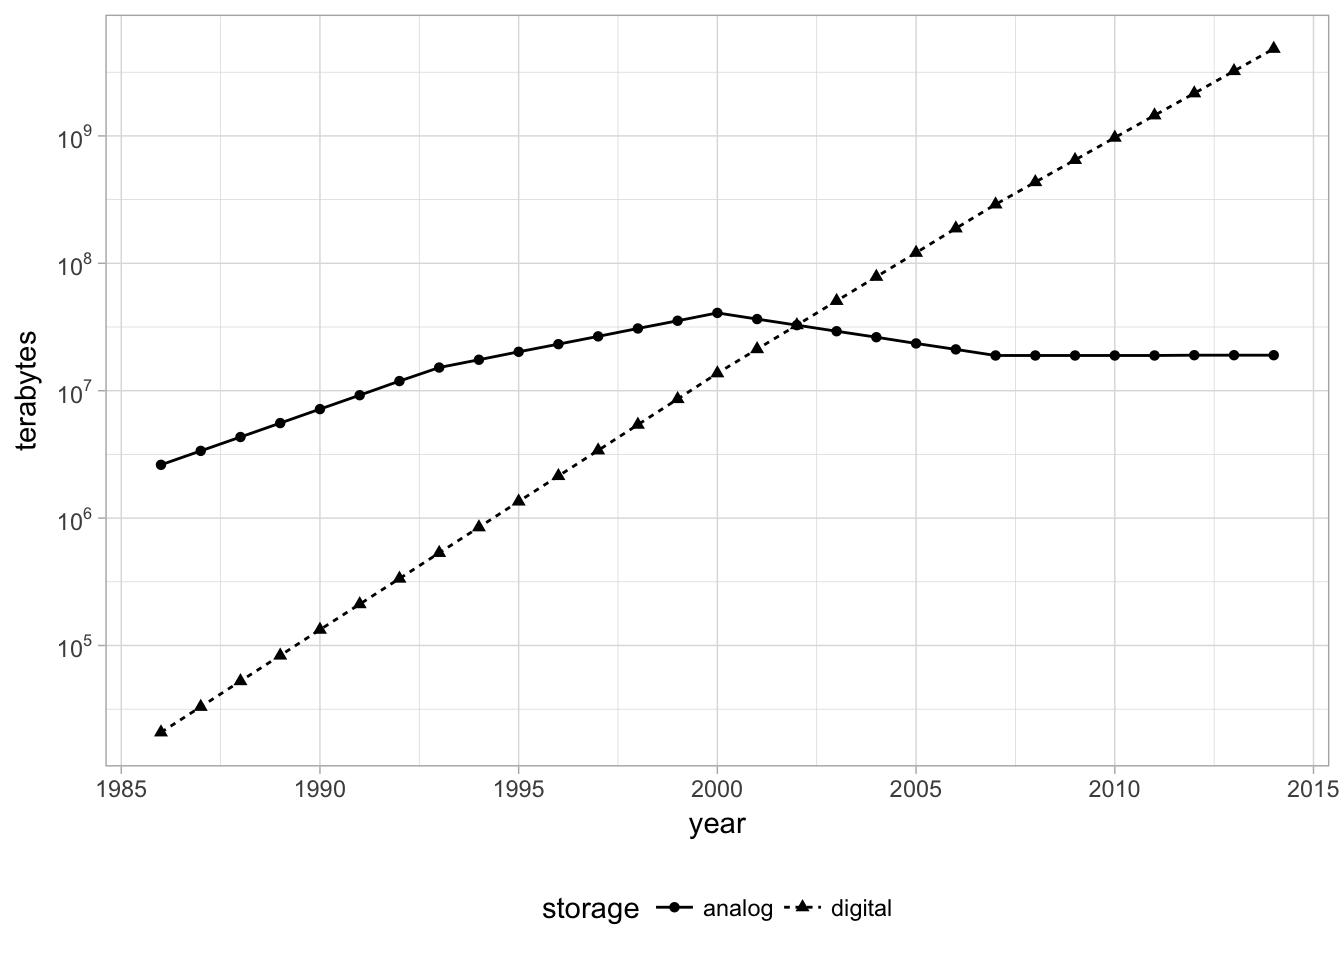
\includegraphics{the-r-in-spark_files/figure-latex/unnamed-chunk-1-1} 

}

\caption{World’s capacity to store information.}\label{fig:unnamed-chunk-1}
\end{figure}

With the ambition to provide a searchable tool to all this new digital
information, many companies attempted to provide such functionality with
what we know today as web search or search engines. Given the vast
amount of digital information, managing information at this scale was a
challenging problem that companies had to tackle. Search engines were
unble to store all the web page information required to support web
searches in a single computer. This meant that they had to split
information across many machines, which was accomlished by splitting
this data and storing it as many files across many machines, this
approach became known as the Google File System from a research paper
published in 2003 by Google \citep{google-file-system}.

One year later, in 2004, Google published a new paper describing how to
perform operations across the Google File System, this approach came to
be known as \textbf{MapReduce} \citep{google-map-reduce}. As you would
expect, there are two operations in MapReduce: Map and Reduce. The
\textbf{map operation} provides an arbitrary way to transform each file
into a new file, usually defined by arbitrary code that scans the file
and outputs a different file. The \textbf{reduce operation} combines two
files into a new one. These two operations are sufficient to process
data at the scale of the data available in the web. For instance, one
could define a mapping operation that splits each word in a text file
and outputs a new file counting occurrence of words; the reduce
operation can be defined to take two word-counting files and combine
them by aggregating the total occurrences for each worf. Once defined, a
cluster implementing MapReduce can perform this operation several times
across many machines to process data at the scale of the entire web.
Counting words is often the most basic example, but MapReduce can be
also used to rank web pages efficietly and many other much more
interesting applications.

After these papers were released by Google, a team in Yahoo worked on
implementing the Google File System and MapReduce as a single open
source project. This project was released in 2006 as \textbf{Hadoop}
implementing MapReduce and the Google File System implemented as the
Hadoop File System, or \textbf{HDFS} for short. The Hadoop project made
distributed file-based computing accessible to a wider range of users
and organizations that made use of MapReduce beyond web data processing.

While Hadoop provided support to perform map/reduce operations over a
distributed file system, it still required each map/reduce operation to
be written with code every time a data analysys was run. The
\textbf{Hive} project, released in 2008 by Facebook, brought Structured
Query Language (SQL) support to Hadoop. This meant that data analysis
could now be performed at large-scale without the need to write code for
each map/reduce operation, but instead, one could write generic data
analysis statements that are much easier to understand and write.

\hypertarget{spark}{%
\section{Spark}\label{spark}}

While Hadoop with Hive was a powerful tool, it was still working over a
distributed file system and was dependent on map/reduce operations. This
meant that it was running using disk drives which tend to be
significantly slower than using a computer's memory. In 2009, the
\textbf{Apache Spark} projects starts in Berkeley to improve over
Hadoop. Specifically, by making use of memory (instead of disk drives)
and by providing a richer set of verbs beyond map/reduce, this allowed
it to be much faster and generic than its predecessor. For instance, one
can
\href{https://databricks.com/blog/2014/11/05/spark-officially-sets-a-new-record-in-large-scale-sorting.html}{sort
100TB of data in 72min and 2100 computers using Hadoop, but only 206
computers in 23min using Spark}. Spark was build using the Scala
programming language, but interfaces to other programming languages are
also provided today. Spark was released as an open source project in
2010 with the scope of the project defined as follows:

\begin{quote}
``Apache Spark is a fast and general engine for large-scale data
processing.''

--- \href{http://spark.apache.org/}{spark.apache.org}
\end{quote}

meaning that Spark is a tool designed to support:

\begin{itemize}
\tightlist
\item
  \textbf{Data Processing}: Data processing is the collection and
  manipulation of items of data to produce meaningful information
  \citep{data-processing}.
\item
  \textbf{Large-Scale}: What \emph{large} means is hard to quantify, but
  one can interpret this as cluster-scale instead, which represents a
  set of connected computers that work together.
\item
  \textbf{General}: Spark optimizes and executes parallel generic code,
  as in, there is no restriction as to what type of code one can write
  in Spark.
\item
  \textbf{Fast}: Spark is much faster than its predecessor by making
  efficient use of memory to speed data access while running algorithms
  at scale.
\end{itemize}

Spark is good at tackling large-scale data processing problems, this
usually known as \textbf{big data}
(\href{https://en.wikipedia.org/wiki/big_data}{data sets that are more
voluminous and complex that traditional ones}), but also is good at
tackling large-scale computation problems, known as \textbf{big compute}
(\href{https://www.nimbix.net/glossary/big-compute/}{tools and
approaches using a large amount of CPU and memory resources in a
coordinated way}). There is a third problem space where data nor compute
are necessarily large scale and yet, there are significant benefits from
using the same tools.

Big data and big compute problems are usually easy to spot, if the data
does not fit into a single machine, you might have a big data problem;
if the data fits into a single machine but a process over the data takes
days, weeks or months to compute, you might have a big compute problem.

For the third problem space, there are a few use cases this breaks to:

\begin{enumerate}
\def\labelenumi{\arabic{enumi}.}
\item
  \textbf{Velocity}: One can have a dataset of 10GB in size and a
  process that takes 30min to run over this data, this is by no means
  big-compute nor big-data; however, if a data scientist is researching
  ways to improve accuracy for their models, reducing the runtime down
  to 3min it's a 10X improvement, this improvement can lead to
  significant advances and productivity gains by increasing the velocity
  at which one can analyze data.
\item
  \textbf{Variety}: One can have an efficient process to collect data
  from many sources into a single location, usually a database, this
  process could be already running efficiently and close to realtime.
  Such processes are known at ETL (Extract-Transform-Load); data is
  extracted from multiple sources, transformed to the required format
  and loaded in a single data store. While this has worked for years,
  the tradeoff from this system is that adding a new data source is
  expensive, the system is centralized and tightly controlled. Since
  making changes to this type of systems could cause the entire process
  to come to a halt, adding new data sources usually takes long to be
  implemented. Instead, one can store all data its natural format and
  process it as needed using cluster computing, this architecture is
  currently known as a
  \href{https://en.wikipedia.org/wiki/Data_lake}{data lake}.
\end{enumerate}

Some people refer to some of these benefits as
\href{http://www.theserverside.com/feature/Handling-the-four-Vs-of-big-data-volume-velocity-variety-and-veracity}{the
four 'V's of big data}: Velocity, Variety, Volume and Veracity (which
asserts that data can vary greatly in quality which require analysis
methods to improve accuracy across a variety of sources). Others have
gone as far as expending this to
\href{https://en.wikipedia.org/wiki/Big_data}{five} or even as
\href{https://tdwi.org/articles/2017/02/08/10-vs-of-big-data.aspx}{the
10 Vs of Big Data}. Mnemonics set aside, cluster computing is being used
today in more innovative ways and and is not uncommon to see
organizations experimenting with new workflows and a variety of tasks
that were traditionally uncommon for cluster computing. Much of the hype
attributed to big data falls into this space, where some will argue that
everything should be considered big data and where others will argue
than nothing should. My hope is that this book will help you understand
the opportunities and limitations of Apache Spark with R.

\hypertarget{r}{%
\section{R}\label{r}}

R is a computing language with it's inception dating back to Bell
Laboratories. John Chambers explained in useR 2016 that at the time,
computing was done by calling Fortran subroutines which, apparently,
were not pleasant to deal with. The S computing language was designed as
an interface language to support higher abstractions to perform
statistical computing over existing subroutines:

\begin{figure}

{\centering 
\includegraphics[width=22.22in]{images/01-intro-s-algorithm-interface} 

}

\caption{Interface language diagram by John Chambers from useR 2016.}\label{fig:s-diagram}
\end{figure}

R is a modern and free implementation of S, specifically:

\begin{quote}
R is a programming language and free software environment for
statistical computing and graphics.

--- \href{https://www.r-project.org/}{The R Project for Statistical
Computing}
\end{quote}

There are two strong arguments for choosing R over other computing
languages while working with data:

\begin{itemize}
\tightlist
\item
  The \textbf{R Language} was designed by statisticians for
  statisticians, meaning, this is one of the few successful languages
  designed for non-programmers; so learning R will probably feel more
  natural. Additionally, since the R language was designed to be an
  interface to other tools and languages, R allows you to focus more on
  modeling and less on the peculiarities of computer science and
  engineering.
\item
  The \textbf{R Community} provides a rich package archive provided by
  CRAN (\href{https://cran.r-project.org/}{The Comprehensive R Archive
  Network}) which allows you to install ready-to-use packages to perform
  many tasks, most notably, high-quality statistic models with many only
  available in R. In addition, the R community is a welcoming and active
  group of talented individuals motivated to help you succeed. Many
  packages provided by the R community make R, by far, the place to do
  statistical computing. To mention some of the popular packages:
  \href{https://CRAN.R-project.org/package=dplyr}{dplyr} to manipulate
  data, \href{https://CRAN.R-project.org/package=cluster}{cluster} to
  analyze clusters and
  \href{https://CRAN.R-project.org/package=ggplot2}{ggplot2} to
  visualize data.
\end{itemize}

One can argue to what degree other fields, like machine learning,
overlap with statistics; so far, most people will argue that the overlap
is non-trivial. Similar arguments can be made for data science, big
data, deep learning and beyond. With the continuous rise of popularity
of R, I can only expect R's influence and scope to keep growing over
time; we can take a look at the historic downloads of R packages in CRAN
to get some sense of R's \protect\hyperlink{cran-downloads}{recent
growth}:

\begin{figure}

{\centering 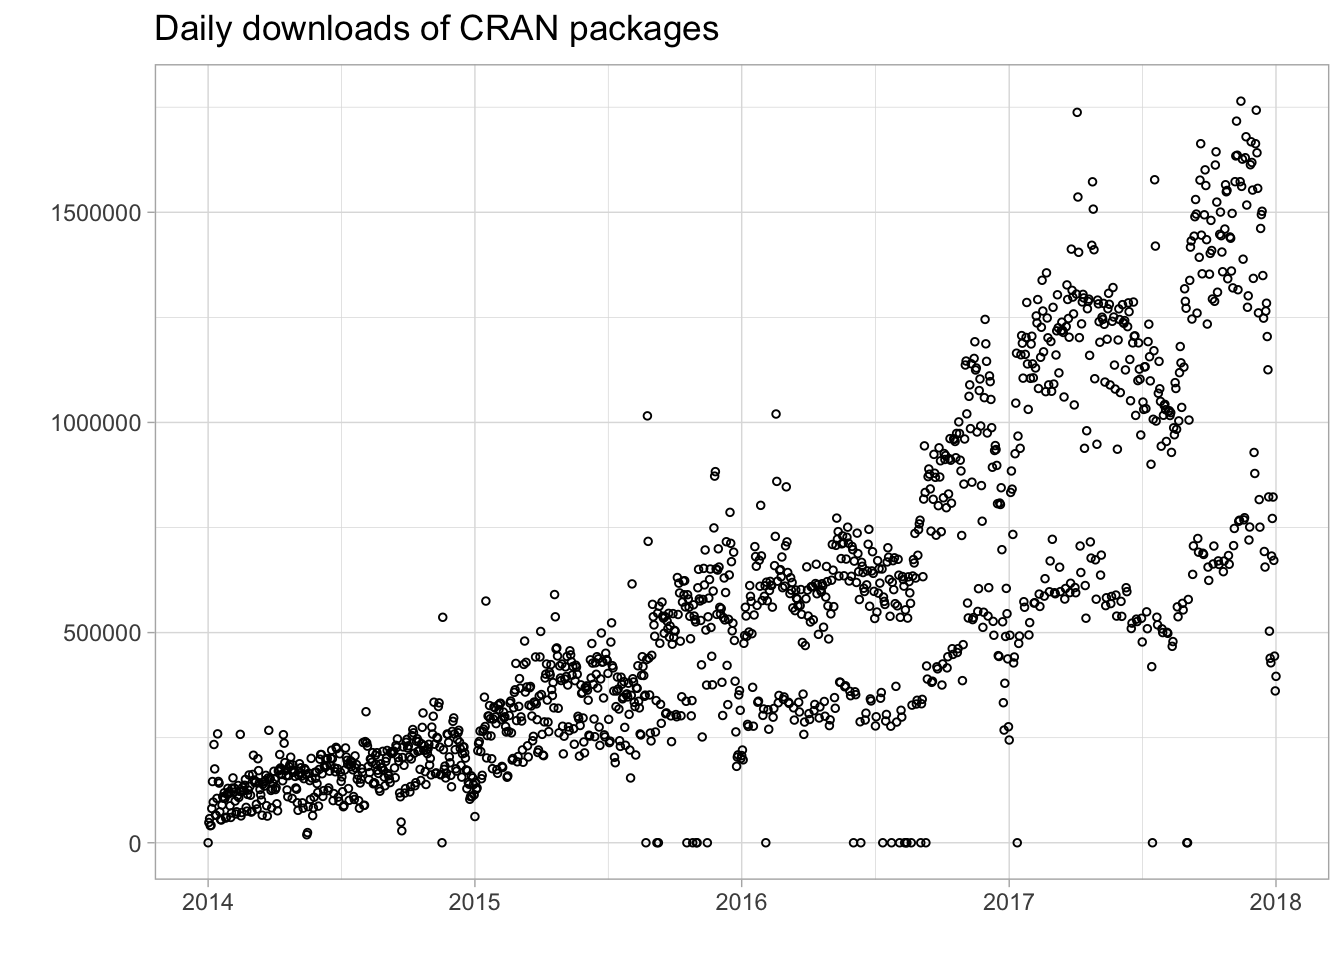
\includegraphics{the-r-in-spark_files/figure-latex/unnamed-chunk-2-1} 

}

\caption{Daily downloads of CRAN packages.}\label{fig:unnamed-chunk-2}
\end{figure}

\hypertarget{sparklyr}{%
\section{sparklyr}\label{sparklyr}}

Back in 2016, there was a need in the R community to support Spark
through an interface compatible with other R packages, easy to use and
available in CRAN. To this end, development of \texttt{sparklyr} started
in 2016 by RStudio under \href{https://github.com/jjallaire}{JJ
Allaire}, \href{https://github.com/kevinushey}{Kevin Ushey} and
\href{https://github.com/javierluraschi}{Javier Luraschi}, version
\href{https://blog.rstudio.com/2016/09/27/sparklyr-r-interface-for-apache-spark/}{0.4
was released} in summer during the \emph{useR!} conference, this first
version added support for \texttt{dplyr}, \texttt{DBI}, modeling with
\texttt{MLlib} and an extensible API that enabled extensions like
\href{https://www.h2o.ai/}{H2O}'s
\href{https://github.com/h2oai/rsparkling/}{rsparkling} package. Since
then, many new features and improvements have been made available
through
\href{https://blog.rstudio.com/2017/01/24/sparklyr-0-5/}{sparklyr 0.5},
\href{https://blog.rstudio.com/2017/07/31/sparklyr-0-6/}{0.6},
\href{https://blog.rstudio.com/2018/01/29/sparklyr-0-7/}{0.7} and
\href{https://blog.rstudio.com/2018/05/14/sparklyr-0-8/}{0.8}.

Officially,

\begin{quote}
\texttt{sparklyr} is an R interface for Apache Spark.

---\href{https://github.com/rstudio/sparklyr}{github.com/rstudio/sparklyr}
\end{quote}

It's available in CRAN and works like any other CRAN package, meaning
that: it's agnostic to Spark versions, it's easy to install, it serves
the R community, it embraces other packages and practices from the R
community and so on. It's hosted in GitHub under
\href{https://github.com/rstudio/sparklyr}{github.com/rstudio/sparklyr}
and licensed under Apache 2.0 which is allows you to clone, modify and
\protect\hyperlink{contributing}{contribute back} to this project.

While thinking of who and why should use \texttt{sparklyr}, the
following roles come to mind:

\begin{itemize}
\tightlist
\item
  \textbf{New Users}: For new users, \texttt{sparklyr} provides the
  easiest way to get started with Spark. My hope is that the first
  chapters of this book will get you up running with ease and set you up
  for long term success.
\item
  \textbf{Data Scientists}: For data scientists that already use and
  love R, \texttt{sparklyr} integrates with many other R practices and
  packages like \texttt{dplyr}, \texttt{magrittr}, \texttt{broom},
  \texttt{DBI}, \texttt{tibble} and many others that will make you feel
  at home while working with Spark. For those new to R and Spark, the
  combination of high-level workflows available in \texttt{sparklyr} and
  low-level extensibility mechanisms make it a productive environment to
  match the needs and skills of every data scientist.
\item
  \textbf{Expert Users}: For those users that are already immersed in
  Spark and can write code natively in Scala, consider making your
  libraries available as an \texttt{sparklyr}
  \protect\hyperlink{writting-extensions}{extension} to the R community,
  a diverse and skilled community that can put your contributions to
  good use while moving
  \href{https://en.wikipedia.org/wiki/Open_science}{open science}
  forward.
\end{itemize}

This book is titled ``The R in Spark'' as a way to describe and teach
that area of overlap between Spark and R. The R package that represents
this overlap is \texttt{sparklyr}; however, the overlap goes beyond a
package. It's an overlap of communities, expectations, future
directions, packages and package extensions as well. Naming this book
\texttt{sparklyr} or ``Introduction to sparklyr'' would have left behind
a much more exciting opportunity, an opportunity to present this book as
an intersection of the R and Spark communities. Both are solving very
similar problems with a set of different skills and backgrounds;
therefore, it is my hope that \texttt{sparklyr} can be a fertile ground
for innovation, a welcoming place to newcomers, a productive place for
experienced data scientists and an open community where cluster
computing and modeling can come together.

Here are some resources to help you get involved:

\begin{itemize}
\tightlist
\item
  \textbf{Documentation}: This should be your entry point to learn more
  about sparklyr, the documentation is kept up to date with examples,
  reference functions and many more relevant resources,
  \url{https://spark.rstudio.com}.
\item
  \textbf{Github}: If you believe something needs to get fixed, open a
  GitHub issue or send us a pull request,
  \url{https://github.com/rstudio/sparklyr}.
\item
  \textbf{Stack Overflow}: For general questions, Stack Overflow is a
  good place to start, \url{stackoverflow.com/tags/sparklyr}.
\item
  \textbf{Gitter}: For urgent issues or to keep in touch you can chat
  with us in Gitter, \url{https://gitter.im/rstudio/sparklyr}.
\end{itemize}

\hypertarget{installation}{%
\chapter{Installation}\label{installation}}

From R, installing and launching a local Spark cluster using
\texttt{sparklyr} is as easy as running:

\begin{Shaded}
\begin{Highlighting}[]
\KeywordTok{spark_install}\NormalTok{()}
\NormalTok{sc <-}\StringTok{ }\KeywordTok{spark_connect}\NormalTok{(}\DataTypeTok{master =} \StringTok{"local"}\NormalTok{)}
\end{Highlighting}
\end{Shaded}

However, to make sure we can all run the code above and understand it,
this chapter will walk you through installing the prerequisites,
installing Spark and connecting to a local Spark cluster.

\hypertarget{prerequisites}{%
\section{Prerequisites}\label{prerequisites}}

As briefly mentioned in the \protect\hyperlink{intro}{Introduction}
chapter, R is a programming language that can run in many platforms and
environments. Most people making use of a programming language also
choose tools to make them more productive in it; for R, RStudio would be
such tool. Strictly speaking, RStudio is an Integrated Development
Environment or IDE for short, which also happens to support many
platforms and environments. R and RStudio are the free software tools
this book will make use of and therefore, I strongly recommend you get
those installed if you haven't done so already.

Additionally, since Spark is build in the Scala programming language
which is run by the Java Virtual Machine, you also need to install Java
7 or newer in your system. It is likely that your system already has
Java installed, but is probably worth updating with the steps bellow.

\hypertarget{install-r}{%
\subsection{Install R}\label{install-r}}

From \href{https://r-project.org/}{r-project.org}, download and launch
the installer for your platform, Windows, Macs or Linux available.

\begin{figure}

{\centering 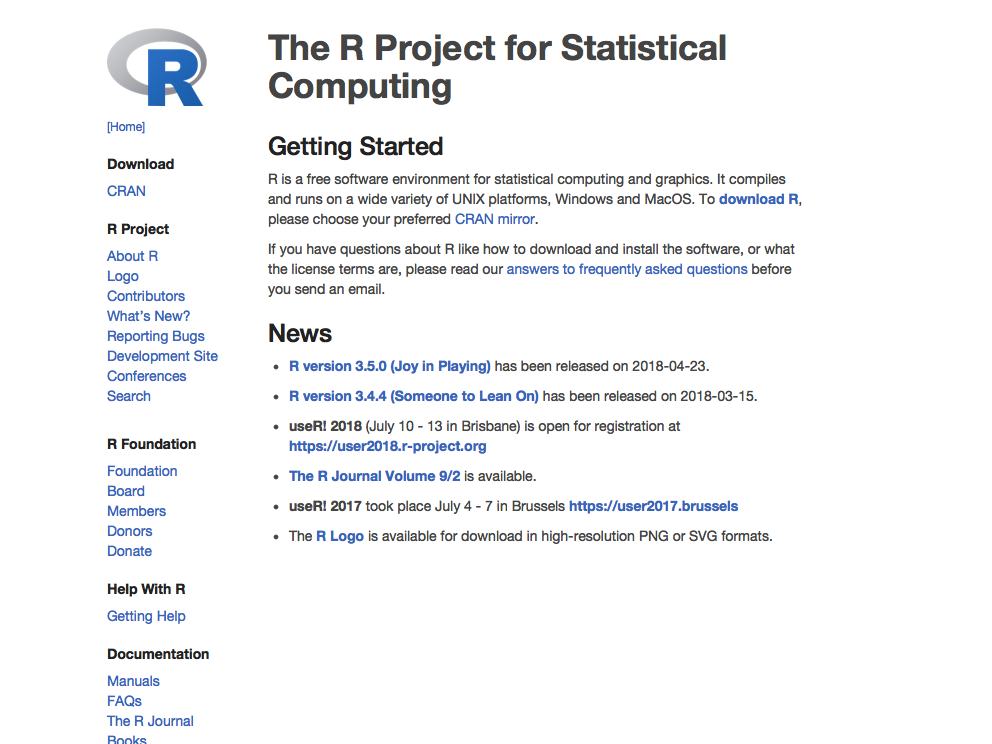
\includegraphics[width=13.78in]{images/02-getting-started-download-r} 

}

\caption{The R Project for Statistical Computing.}\label{fig:r-download}
\end{figure}

\hypertarget{install-java}{%
\subsection{Install Java}\label{install-java}}

From
\href{http://www.oracle.com/technetwork/java/javase/downloads/jdk8-downloads-2133151.html}{oracle.com/technetwork/java/javase/downloads/jdk8-downloads-2133151.html},
download and launch the installer for your platform, Windows, Macs or
Linux available. While installing the JRE (Java Runtime Environment) is
sufficient for most operations, in order to build extensions you will
need the JDK (Java Developer Kit); therefore, I rather recommend
installing the JDK in the first place.

\begin{figure}

{\centering 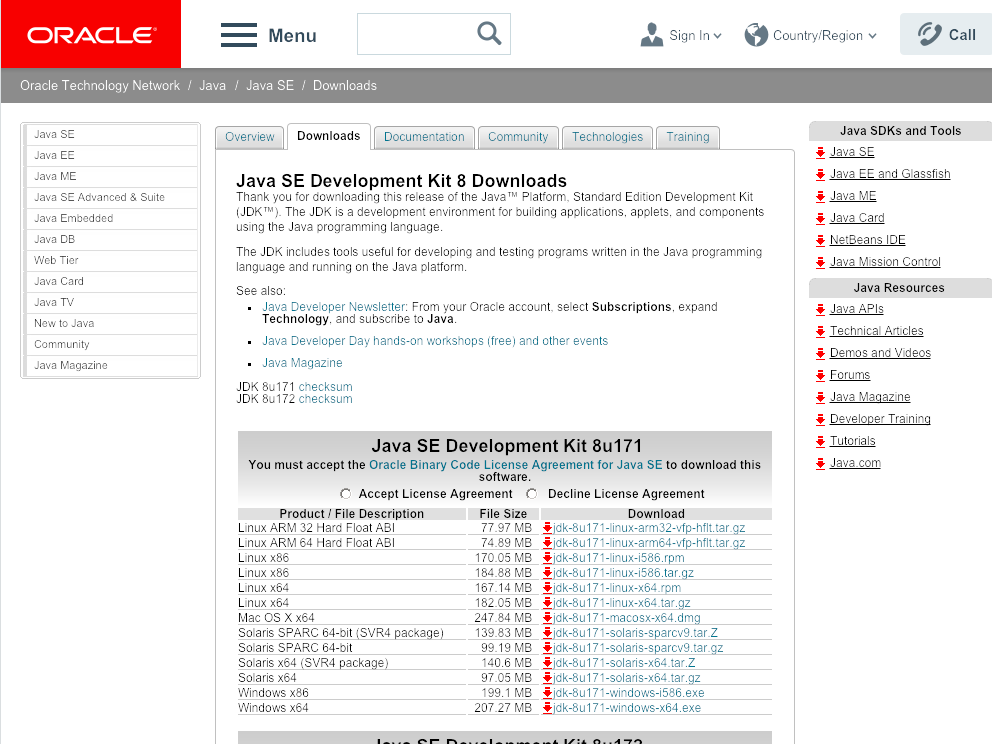
\includegraphics[width=13.78in]{images/02-getting-started-jdk-8} 

}

\caption{Java Download.}\label{fig:java-download}
\end{figure}

Starting with Spark 2.1, Java 8 is required; however, previous versions
of Spark support Java 7. Regardless, we recommend installing Java 8 as
described in this chapter

\hypertarget{install-rstudio}{%
\subsection{Install RStudio}\label{install-rstudio}}

While installing RStudio is not strictly required to work with
\texttt{sparklyr} in R, it will make you much more productive and
therefore, I would recommend you take the time to install RStudio from
\href{https://www.rstudio.com/products/rstudio/download/}{rstudio.com/products/rstudio/download/},
then download and launch the installer for your platform: Windows, Macs
or Linux.

\begin{figure}

{\centering 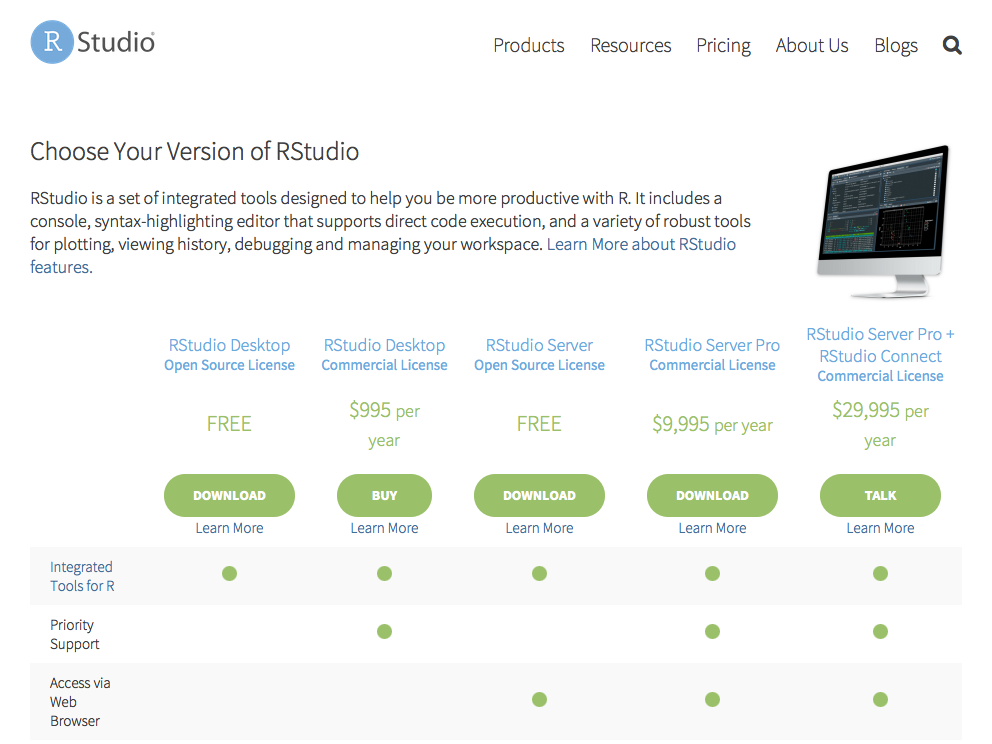
\includegraphics[width=13.78in]{images/02-getting-started-rstudio} 

}

\caption{RStudio Downloads.}\label{fig:rstudio-download}
\end{figure}

After launching RStudio, identify the Console panel since this is where
most of the code will be executed in this book. For additional learning
resources on R and RStudio consider visiting:
\href{https://www.rstudio.com/online-learning/}{rstudio.com/online-learning/}.

\hypertarget{install-sparklyr}{%
\subsection{Install sparklyr}\label{install-sparklyr}}

First of all, we would want to install \texttt{sparkylr}. As many other
R packages, \texttt{sparklyr} is available in
\href{https://CRAN.R-project.org/package=sparklyr}{CRAN} and can be
easily installed as follows:

\begin{Shaded}
\begin{Highlighting}[]
\KeywordTok{install.packages}\NormalTok{(}\StringTok{"sparklyr"}\NormalTok{)}
\end{Highlighting}
\end{Shaded}

The CRAN release of \texttt{sparklyr} contains the most stable version
and it's the recommended version to use; however, for those that need or
might want to try newer features being developed in \texttt{sparklyr}
you can install directly from GitHub using the \texttt{devtools}
package. First install the \texttt{devtools} package and then
\texttt{sparklyr} as follows:

\begin{Shaded}
\begin{Highlighting}[]
\KeywordTok{install.packages}\NormalTok{(}\StringTok{"devtools"}\NormalTok{)}
\NormalTok{devtools}\OperatorTok{::}\KeywordTok{install_github}\NormalTok{(}\StringTok{"rstudio/sparklyr"}\NormalTok{)}
\end{Highlighting}
\end{Shaded}

\hypertarget{installing-spark}{%
\section{Installing Spark}\label{installing-spark}}

Start by loading \texttt{sparklyr},

\begin{Shaded}
\begin{Highlighting}[]
\KeywordTok{library}\NormalTok{(sparklyr)}
\end{Highlighting}
\end{Shaded}

This will makes all \texttt{sparklyr} functions available in R, which is
really helpful; otherwise, we would have to run each \texttt{sparklyr}
command prefixed with \texttt{sparklyr::}.

As mentioned, Spark can be easily installed by running
\texttt{spark\_install()}; this will install the latest version of Spark
locally in your computer, go ahead and run \texttt{spark\_install()}.
Notice that this command requires internet connectivity to download
Spark.

\begin{Shaded}
\begin{Highlighting}[]
\KeywordTok{spark_install}\NormalTok{()}
\end{Highlighting}
\end{Shaded}

All the versions of Spark that are available for installation can be
displayed with \texttt{spark\_available\_versions()}:

\begin{Shaded}
\begin{Highlighting}[]
\KeywordTok{spark_available_versions}\NormalTok{()}
\end{Highlighting}
\end{Shaded}

\begin{verbatim}
##    spark
## 1  1.6.3
## 2  1.6.2
## 3  1.6.1
## 4  1.6.0
## 5  2.0.0
## 6  2.0.1
## 7  2.0.2
## 8  2.1.0
## 9  2.1.1
## 10 2.2.0
## 11 2.2.1
## 12 2.3.0
\end{verbatim}

A specific version can be installed using the Spark version and,
optionally, by also specifying the Hadoop version. For instance, to
install Spark 1.6.3, we would run \texttt{spark\_install("1.6.3")}.

You can also check which versions are installed by running:

\begin{Shaded}
\begin{Highlighting}[]
\KeywordTok{spark_installed_versions}\NormalTok{()}
\end{Highlighting}
\end{Shaded}

Finally, in order to uninstall an specific version of Spark you can run
\texttt{spark\_uninstall()} by specifying the Spark and Hadoop versions,
for instance:

\begin{Shaded}
\begin{Highlighting}[]
\KeywordTok{spark_uninstall}\NormalTok{(}\DataTypeTok{version =} \StringTok{"1.6.0"}\NormalTok{, }\DataTypeTok{hadoop =} \StringTok{"2.6"}\NormalTok{)}
\end{Highlighting}
\end{Shaded}

\hypertarget{connecting-to-spark}{%
\section{Connecting to Spark}\label{connecting-to-spark}}

It's important to mention that, so far, we've only installed a local
Spark cluster. A local cluster is really helpful to get started, test
code and troubleshoot with ease; further chapters will explain where to
find, install and connect to real Spark clusters with many machines; but
for the first few chapters, we will focus on using local clusters.

Threfore, to connect to this local cluster we simple run:

\begin{Shaded}
\begin{Highlighting}[]
\NormalTok{sc <-}\StringTok{ }\KeywordTok{spark_connect}\NormalTok{(}\DataTypeTok{master =} \StringTok{"local"}\NormalTok{)}
\end{Highlighting}
\end{Shaded}

The \texttt{master} parameter helps \texttt{sparklyr} find which is the
``main'' machine from the Spark cluster, this machine is often call the
driver node. While working with real clusters using many machines, most
machines will be worker machines and one will be the master. Since we
only have a local cluster with only one machine, we will default to use
\texttt{"local"} for now.

\hypertarget{using-spark}{%
\section{Using Spark}\label{using-spark}}

Now that you are connected, we can run a simple commands. For instance,
let's start by loading some text.

First, lets create a text file by running:

\begin{Shaded}
\begin{Highlighting}[]
\KeywordTok{write}\NormalTok{(}\StringTok{"Hello World!"}\NormalTok{, }\StringTok{"hello.txt"}\NormalTok{)}
\end{Highlighting}
\end{Shaded}

Which we can read back in Spark by running:

\begin{Shaded}
\begin{Highlighting}[]
\KeywordTok{spark_read_text}\NormalTok{(sc, }\StringTok{"hello"}\NormalTok{, }\StringTok{"hello.txt"}\NormalTok{)}
\end{Highlighting}
\end{Shaded}

\begin{verbatim}
## # Source:   table<hello> [?? x 1]
## # Database: spark_connection
##   line        
##   <chr>       
## 1 Hello World!
\end{verbatim}

\hypertarget{spark-web-interface}{%
\subsection{Web Interface}\label{spark-web-interface}}

Most of the Spark commands will get started from the R console; however,
it is often the case that monitoring and analizing execution is done
through Spark's web interface. This interface is a web page provided by
the driver node which can be accessed from \texttt{sparklyr} by running:

\begin{Shaded}
\begin{Highlighting}[]
\KeywordTok{spark_web}\NormalTok{(sc)}
\end{Highlighting}
\end{Shaded}

\begin{figure}

{\centering 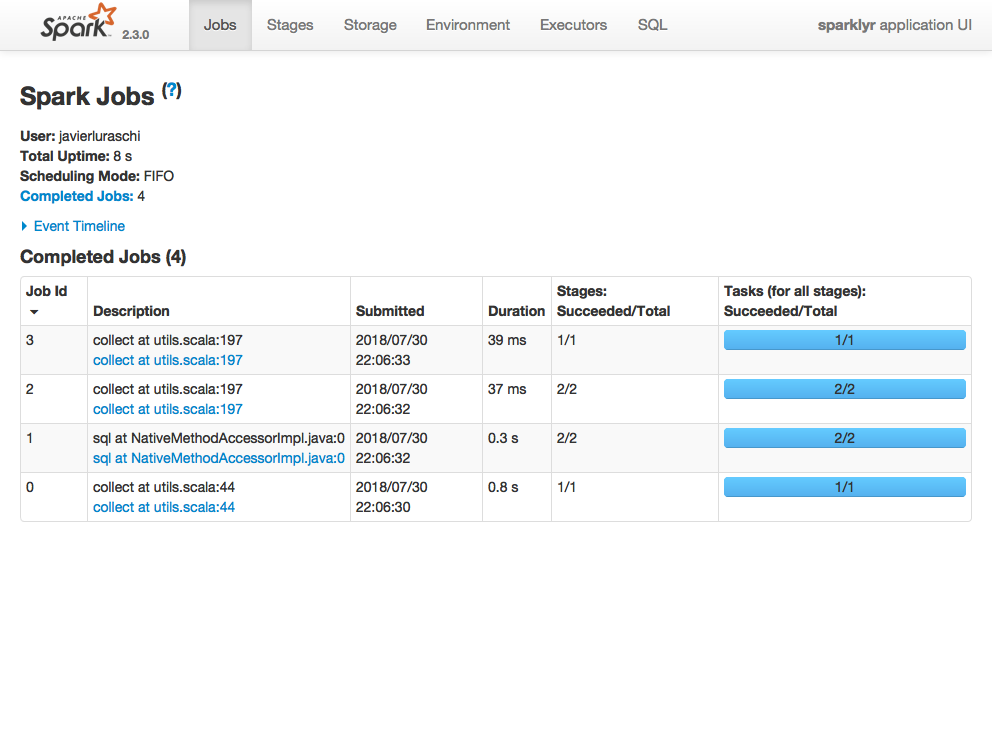
\includegraphics[width=13.78in]{images/02-getting-started-spark-web} 

}

\caption{Apache Spark Web Interface.}\label{fig:spark-web}
\end{figure}

\hypertarget{logs}{%
\subsection{Logs}\label{logs}}

Another common tool is to read through the Spark logs, a log is just a
text file where Spark will append information relevant to the execution
of tasks in the cluster. For local clusters, we can retrieve the
\texttt{sparklyr} related log entries by running:

\begin{Shaded}
\begin{Highlighting}[]
\KeywordTok{spark_log}\NormalTok{(sc, }\DataTypeTok{filter =} \StringTok{"sparklyr"}\NormalTok{, }\DataTypeTok{n =} \DecValTok{5}\NormalTok{)}
\end{Highlighting}
\end{Shaded}

\begin{verbatim}
## 18/07/16 10:21:20 INFO SparkContext: Submitted application: sparklyr
## 18/07/16 10:21:20 INFO SparkContext: Added JAR file:/Library/Frameworks/R.framework/Versions/3.5/Resources/library/sparklyr/java/sparklyr-2.3-2.11.jar at spark://localhost:55314/jars/sparklyr-2.3-2.11.jar with timestamp 1531761680925
## 18/07/16 10:21:24 INFO Executor: Fetching spark://localhost:55314/jars/sparklyr-2.3-2.11.jar with timestamp 1531761680925
## 18/07/16 10:21:24 INFO Utils: Fetching spark://localhost:55314/jars/sparklyr-2.3-2.11.jar to /private/var/folders/fz/v6wfsg2x1fb1rw4f6r0x4jwm0000gn/T/spark-ec1df593-9e04-4ccb-a7d7-1ef2d1e57904/userFiles-048b9d91-c9da-41f3-a301-a399cf1fce20/fetchFileTemp8702458663170880290.tmp
## 18/07/16 10:21:24 INFO Executor: Adding file:/private/var/folders/fz/v6wfsg2x1fb1rw4f6r0x4jwm0000gn/T/spark-ec1df593-9e04-4ccb-a7d7-1ef2d1e57904/userFiles-048b9d91-c9da-41f3-a301-a399cf1fce20/sparklyr-2.3-2.11.jar to class loader
\end{verbatim}

\hypertarget{using-spark-from-rstudio}{%
\subsection{RStudio}\label{using-spark-from-rstudio}}

\textbf{TODO:} Explain and show a couple integration points for those
using \texttt{sparklyr} from RStudio.

\hypertarget{disconnecting}{%
\section{Disconnecting}\label{disconnecting}}

For local clusters and, really, any cluster; once you are done
processing data you should disconnect by running:

\begin{Shaded}
\begin{Highlighting}[]
\KeywordTok{spark_disconnect}\NormalTok{(sc)}
\end{Highlighting}
\end{Shaded}

this will terminate the connection to the cluster but also terminate the
cluster tasks as well. If multiple Spark connections are active, or if
the conneciton instance \texttt{sc} is no longer available, you can also
disconnect all your Spark connections by running
\texttt{spark\_disconnect\_all()}.

\hypertarget{recap}{%
\section{Recap}\label{recap}}

This chapter walked you through installing R, Java, RStudio and
\texttt{sparklyr} as the main tools required to use Spark from R. We
covered installing local Spark clusters using \texttt{spark\_install()}
and learned how to launch the web interface using
\texttt{spark\_web(sc)} and view logs using \texttt{spark\_log(sc)}.

It is my hope that this chapter will help anyone interested in learning
cluster computing using Spark and R to get you started, ready to
experiment on your own and ready to tackle actual data analysis and
modeling tasks without any makor blockers. However, if you hit any
installation or connection issues, start by browsing online for the
error message or open a GitHub issue under
\url{https://github.com/rstudio/sparklyr/issues} to help you get going.

\hypertarget{dplyr}{%
\chapter{Analysis}\label{dplyr}}

While \textbf{this chatper has not been written}, a few resources and
basic examples were made available to help out until this chapter is
written.

\hypertarget{dplyr-1}{%
\section{dplyr}\label{dplyr-1}}

Using \texttt{sparklyr}, you can apply the same data analysis techniques
described in \href{http://r4ds.had.co.nz/transform.html}{Chapter 5 -
Data transformation - R for Data Science} by Garrett Grolemund and
Hadley Wickham.

Once you understand \texttt{dplyr}, you can make use of \texttt{dplyr}
and \texttt{sparklyr} as follows:

\begin{Shaded}
\begin{Highlighting}[]
\KeywordTok{library}\NormalTok{(sparklyr)}
\KeywordTok{library}\NormalTok{(dplyr)}

\CommentTok{# Connect to Spark}
\NormalTok{sc <-}\StringTok{ }\KeywordTok{spark_connect}\NormalTok{(}\DataTypeTok{master =} \StringTok{"local"}\NormalTok{)}

\CommentTok{# Use dplyr's copy_to() to copy the iris dataset to Spark}
\NormalTok{iris_tbl <-}\StringTok{ }\KeywordTok{copy_to}\NormalTok{(sc, iris, }\DataTypeTok{overwrite =} \OtherTok{TRUE}\NormalTok{)}

\CommentTok{# The iris_tbl is a Spark data frame compatible with dplyr}
\NormalTok{iris_tbl}
\end{Highlighting}
\end{Shaded}

\begin{verbatim}
## # Source:   table<iris> [?? x 5]
## # Database: spark_connection
##    Sepal_Length Sepal_Width Petal_Length Petal_Width Species
##           <dbl>       <dbl>        <dbl>       <dbl> <chr>  
##  1          5.1         3.5          1.4         0.2 setosa 
##  2          4.9         3            1.4         0.2 setosa 
##  3          4.7         3.2          1.3         0.2 setosa 
##  4          4.6         3.1          1.5         0.2 setosa 
##  5          5           3.6          1.4         0.2 setosa 
##  6          5.4         3.9          1.7         0.4 setosa 
##  7          4.6         3.4          1.4         0.3 setosa 
##  8          5           3.4          1.5         0.2 setosa 
##  9          4.4         2.9          1.4         0.2 setosa 
## 10          4.9         3.1          1.5         0.1 setosa 
## # ... with more rows
\end{verbatim}

\begin{Shaded}
\begin{Highlighting}[]
\CommentTok{# Transform iris_tbl with dplyr as usual}
\NormalTok{iris_tbl }\OperatorTok\StringTok{ }
\StringTok{  }\KeywordTok{group_by}\NormalTok{(Species) }\OperatorTok\StringTok{ }
\StringTok{  }\KeywordTok{summarise_all}\NormalTok{(}\KeywordTok{funs}\NormalTok{(mean))}
\end{Highlighting}
\end{Shaded}

\begin{verbatim}
## # Source:   lazy query [?? x 5]
## # Database: spark_connection
##   Species    Sepal_Length Sepal_Width Petal_Length Petal_Width
##   <chr>             <dbl>       <dbl>        <dbl>       <dbl>
## 1 versicolor         5.94        2.77         4.26       1.33 
## 2 virginica          6.59        2.97         5.55       2.03 
## 3 setosa             5.01        3.43         1.46       0.246
\end{verbatim}

To understand \texttt{dplyr} further, I would recommend taking a look at
the following vignettes:

\begin{itemize}
\tightlist
\item
  \href{https://cran.r-project.org/web/packages/dplyr/vignettes/dplyr.html}{Introduction
  to dplyr}
\item
  \href{https://cran.r-project.org/web/packages/dplyr/vignettes/two-table.html}{Two-table
  verbs}
\item
  \href{https://cran.r-project.org/web/packages/dplyr/vignettes/window-functions.html}{Window
  functions}
\item
  \href{https://cran.r-project.org/web/packages/dplyr/vignettes/programming.html}{Programming
  with dplyr}
\end{itemize}

\hypertarget{dbi}{%
\section{DBI}\label{dbi}}

The \texttt{DBI} provides an database interface for R, meaning, if you
are familiar with SQL, you can make use of \texttt{DBI} to perform SQL
queries in Spark using \texttt{sparklyr}. To learn more about
\texttt{DBI}, I would recommend reading first
\href{https://cran.r-project.org/web/packages/DBI/vignettes/DBI-1.html}{A
Common Database Interface (DBI)}. Once you are familiar with
\texttt{DBI}, you can use this package with \texttt{sparklyr} as
follows:

\begin{Shaded}
\begin{Highlighting}[]
\KeywordTok{library}\NormalTok{(DBI)}

\KeywordTok{dbGetQuery}\NormalTok{(sc,}
  \StringTok{"SELECT mean(Sepal_Length), mean(Sepal_Width), }
\StringTok{          mean(Petal_Length), mean(Petal_Width)}
\StringTok{   FROM iris}
\StringTok{   GROUP BY Species"}\NormalTok{)}
\end{Highlighting}
\end{Shaded}

\begin{verbatim}
##   avg(Sepal_Length) avg(Sepal_Width) avg(Petal_Length) avg(Petal_Width)
## 1             5.936            2.770             4.260            1.326
## 2             6.588            2.974             5.552            2.026
## 3             5.006            3.428             1.462            0.246
\end{verbatim}

More advanced \texttt{DBI} resources are available in the following
vignettes:

\begin{itemize}
\tightlist
\item
  \href{https://cran.r-project.org/web/packages/DBI/vignettes/DBI-proposal.html}{A
  Common Interface to Relational Databases from R and S -- A Proposal}
\item
  \href{https://cran.r-project.org/web/packages/DBI/vignettes/backend.html}{Implementing
  a new backend}
\item
  \href{https://cran.r-project.org/web/packages/DBI/vignettes/spec.html}{DBI
  specification}
\end{itemize}

\hypertarget{modeling}{%
\chapter{Modeling}\label{modeling}}

While \textbf{this chatper has not been written}, a few resources and
basic examples were made available to help out until this chapter is
written.

\hypertarget{overview}{%
\section{Overview}\label{overview}}

MLlib is Apache Spark's scalable machine learning library and is
available through \texttt{sparklyr}, mostly, with functions prefixed
with \texttt{ml\_}. The following table describes some of the modeling
algorithms supported:

\begin{longtable}[]{@{}ll@{}}
\toprule
Algorithm & Function\tabularnewline
\midrule
\endhead
Accelerated Failure Time Survival Regression &
ml\_aft\_survival\_regression\tabularnewline
Alternating Least Squares Factorization & ml\_als\tabularnewline
Correlation Matrix & ml\_corr\tabularnewline
Decision Trees & ml\_decision\_tree\tabularnewline
Generalized Linear Regression &
ml\_generalized\_linear\_regression\tabularnewline
Gradient-Boosted Trees & ml\_gradient\_boosted\_trees\tabularnewline
Isotonic Regression & ml\_isotonic\_regression\tabularnewline
K-Means Clustering & ml\_kmeans\tabularnewline
Latent Dirichlet Allocation & ml\_lda\tabularnewline
Linear Regression & ml\_linear\_regression\tabularnewline
Linear Support Vector Machines & ml\_linear\_svc\tabularnewline
Logistic Regression & ml\_logistic\_regression\tabularnewline
Multilayer Perceptron & ml\_multilayer\_perceptron\tabularnewline
Naive-Bayes & ml\_naive\_bayes\tabularnewline
One vs Rest & ml\_one\_vs\_rest\tabularnewline
Principal Components Analysis & ml\_pca\tabularnewline
Random Forests & ml\_random\_forest\tabularnewline
Survival Regression & ml\_survival\_regression\tabularnewline
\bottomrule
\end{longtable}

Here is an example to get you started with K-Means:

\begin{Shaded}
\begin{Highlighting}[]
\KeywordTok{library}\NormalTok{(sparklyr)}

\CommentTok{# Connect to Spark in local mode}
\NormalTok{sc <-}\StringTok{ }\KeywordTok{spark_connect}\NormalTok{(}\DataTypeTok{master =} \StringTok{"local"}\NormalTok{)}

\CommentTok{# Copy iris to Spark}
\NormalTok{iris_tbl <-}\StringTok{ }\KeywordTok{sdf_copy_to}\NormalTok{(sc, iris, }\DataTypeTok{overwrite =} \OtherTok{TRUE}\NormalTok{)}

\CommentTok{# Run K-Means for Species using only Petal_Width and Petal_Length as features}
\NormalTok{iris_tbl }\OperatorTok
\StringTok{  }\KeywordTok{ml_kmeans}\NormalTok{(}\DataTypeTok{centers =} \DecValTok{3}\NormalTok{, Species }\OperatorTok{~}\StringTok{ }\NormalTok{Petal_Width }\OperatorTok{+}\StringTok{ }\NormalTok{Petal_Length)}
\end{Highlighting}
\end{Shaded}

\begin{verbatim}
## K-means clustering with 3 clusters
## 
## Cluster centers:
##   Petal_Width Petal_Length
## 1    1.359259     4.292593
## 2    0.246000     1.462000
## 3    2.047826     5.626087
## 
## Within Set Sum of Squared Errors =  31.41289
\end{verbatim}

More examples are reosurces are available in
\href{http://spark.rstudio.com/mlib/}{spark.rstudio.com/mlib}.

\hypertarget{pipelines}{%
\section{Pipelines}\label{pipelines}}

Spark's ML Pipelines provide a way to easily combine multiple
transformations and algorithms into a single workflow, or pipeline.

Take a look at
\href{http://spark.rstudio.com/guides/pipelines/}{spark.rstudio.com/guides/pipelines}
to learn about their purpose and functionality.

\hypertarget{clusters}{%
\chapter{Clusters}\label{clusters}}

Previous chapters focused on using Spark over a single computing
instance, your personal computer. In this chapter we will introduce
techniques to run Spark over multiple computing instances, also known as
a computing cluster, to analyze data at scale.

If you already have a Spark cluster in your organization, you could
consider skipping to the next chapter,
\protect\hyperlink{connections-1}{Connections}, which will teach you how
to connect to an existing cluster.

If don't have a cluster or are considering improvements to your existing
infrastructure, this chapter will introduce some of the cluster trends,
managers and providers available today.

\hypertarget{overview-1}{%
\section{Overview}\label{overview-1}}

There are three major trends in cluster computing worth discussing:
\textbf{on-premise}, \textbf{cloud computing} and \textbf{kubernetes}.
Framing these trends over time will help us understand how they came to
be, what they are and what their future might be:

\begin{figure}

{\centering \includegraphics[width=1\linewidth]{the-r-in-spark_files/figure-latex/unnamed-chunk-21-1} 

}

\caption{Google trends for on-premise (mainframe), cloud computing and kubernetes.}\label{fig:unnamed-chunk-21}
\end{figure}

For \textbf{on-premise} clusters, someone, either yourself or someone in
your organiation purchased physical computers that are intended to be
used for cluster computing. The computers in this cluster can made of
\emph{off-the-shelf} hardware, meaning that someone placed an order to
purchase computers usually found in stores shelves or,
\emph{high-performance} hardware, meaning that a computing vendor
provided highly customized computing hardware which also comes optimized
for high-performance network connectivity, power consumption, etc. When
purchasing hundreds or thousands of computing instances, it doesn't make
sense to keep them in the usual computing case that we are all familiar
with, but rather, it makes sense to stack them as efficient as possible
on top of each other to minimize room space. This group of efficiently
stacked computing instances is known as a
\href{https://en.wikipedia.org/wiki/Rack_unit}{rack}. Once a cluster
grows to thousands of computers, you will also need to host hundreds of
racks of computing devices, at this scale, you would also need
significant physical space to hosts those racks. A building that
provides racks of computing instances is usually known as a
\emph{data-center}. At the scale of a data center, optimizing the
building that holds them, their heating system, power suply, network
connectivity, etc. becomes also relevant to optimize. In 2011, Facebook
\href{https://code.facebook.com/posts/187637061409082/building-efficient-data-centers-with-the-open-compute-project/}{announced}
the \href{http://www.opencompute.org/}{Open Compute Project} inniciative
which provides a set of data center blueprints free for anyone to use.

There is nothing preventing us from building our own data centers and in
fact, many organizations have followed this path. For instance, Amazon
started as an online book store, over the years Amazon grew to sell much
more than just books and, with it's online store growth, their data
centers also grew in size. In 2002, Amazon considered
\href{https://en.wikipedia.org/wiki/Amazon_Web_Services\#History}{selling
access to virtual servers}, in their data centers to the public and, in
2004, Amazon Web Services launched as a way to let anyone rent a subset
of their datacenters on-demand, meaning that one did not have to
purchase, configure, maintain nor teardown it's own clusters but could
rather rent them from Amazon directly.

The on-demand compute model is what we know today as \textbf{Cloud
Computing}. It's a concept that evolved from Amazon Web Services
providing their data centers as a service. In the cloud, the cluster you
use is not owned by you and is neither in your physical building, but
rather, it's a data center owned and managed by someone else. Today,
there are many cloud providers in this space ranging from Amazon,
Microsoft, Google, IBM and many others. Most cloud computing platforms
provide a user interface either through a web applciation and command
line to request and manage resources.

While the bennefits of processing data in the \emph{cloud} were obvious
for many years, picking a cloud provider had the unintended side-effect
of locking organizations with one particular provider, making it hard to
switch between provideers or back to on-premise clusters.
\textbf{Kubernetes}, announced by Google in 2014, is an
\href{https://github.com/kubernetes/kubernetes/}{open source system for
managing containerized applications across multiple hosts}. In practice,
it provides common infrastructure otherwise proprietary to cloud
providers making it much easier to deploy across multiple cloud
providers and on-premise as well. However, being a much newer paradigm
than on-premise or cloud computing, it is still in it's adoption phase
but, nevertheless, promising for cluster computing in general and,
specifically, for Apache Spark.

\hypertarget{managers}{%
\section{Managers}\label{managers}}

In order to run Spark within a computing cluster, one needs to run
something capable of initializing Spark over each compute instance, this
is known as a
\href{https://en.wikipedia.org/wiki/Cluster_manager}{cluster manager}.
The available cluster managers in Spark are: \textbf{Spark Standalone},
\textbf{YARN}, \textbf{Mesos} and \textbf{Kubernetes}.

\hypertarget{clusters-standalone}{%
\subsection{Standalone}\label{clusters-standalone}}

In \textbf{Spark Standalone}, Spark works on it's own without additional
software requirements since it provides it's own cluster manager as part
of the Spark installation.

\begin{figure}

{\centering 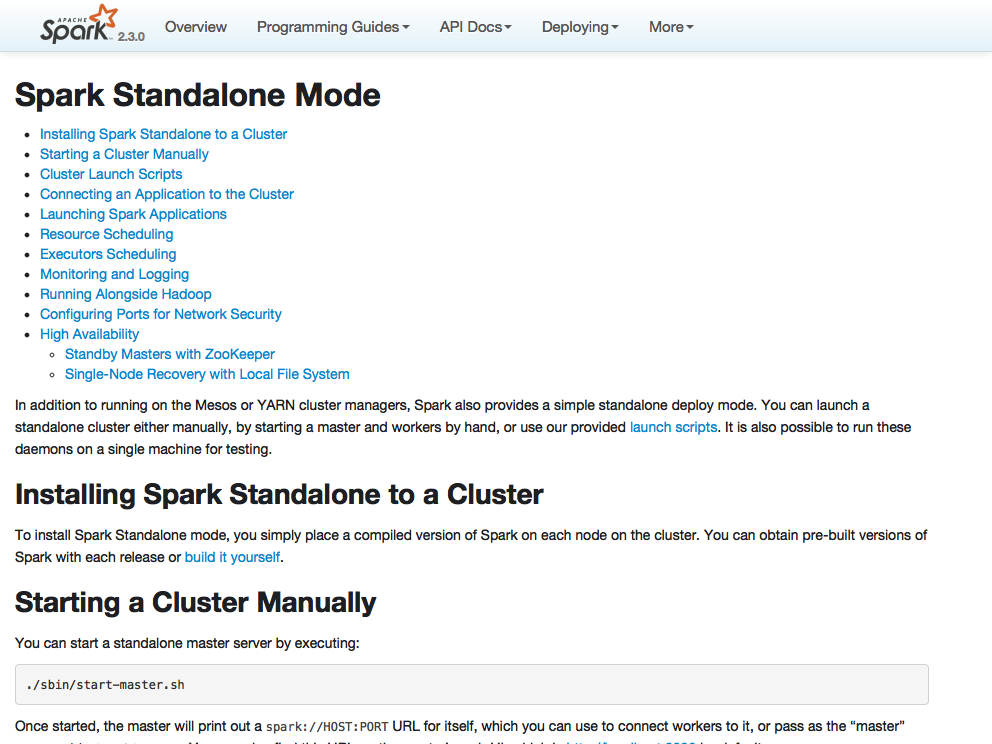
\includegraphics[width=13.78in]{images/05-clusters-spark-standalone} 

}

\caption{Spark Standalone Site.}\label{fig:spark-standalone}
\end{figure}

By completing the \protect\hyperlink{installation}{Installation}
chapter, you should have a local Spark installation available, which we
can use to initialize a local stanalone Spark cluster. First, retrieve
the \texttt{SPARK\_HOME} directory by running
\texttt{sparklyr::spark\_home\_dir()} from R and then, from a terminal
or R, use \texttt{start-master.sh} and \texttt{start-slave.sh} as
follows:

\begin{Shaded}
\begin{Highlighting}[]
\CommentTok{# Retrieve the Spark installation directory}
\NormalTok{spark_home <-}\StringTok{ }\NormalTok{sparklyr}\OperatorTok{::}\KeywordTok{spark_home_dir}\NormalTok{()}

\CommentTok{# Build path to start-master.sh}
\NormalTok{start_master <-}\StringTok{ }\KeywordTok{file.path}\NormalTok{(spark_home, }\StringTok{"sbin"}\NormalTok{, }\StringTok{"start-master.sh"}\NormalTok{)}

\CommentTok{# Execute start-master.sh to start the cluster manager master node}
\KeywordTok{system2}\NormalTok{(start_master)}

\CommentTok{# Build path to start-slave}
\NormalTok{start_slave <-}\StringTok{ }\KeywordTok{file.path}\NormalTok{(spark_home, }\StringTok{"sbin"}\NormalTok{, }\StringTok{"start-slave.sh"}\NormalTok{)}

\CommentTok{# Execute start-slave.sh to start a worker and register in master node}
\KeywordTok{system2}\NormalTok{(start_slave, }\KeywordTok{paste0}\NormalTok{(}\StringTok{"spark://"}\NormalTok{, }\KeywordTok{system2}\NormalTok{(}\StringTok{"hostname"}\NormalTok{, }\DataTypeTok{stdout =} \OtherTok{TRUE}\NormalTok{), }\StringTok{":7077"}\NormalTok{))}
\end{Highlighting}
\end{Shaded}

The previous command initialized the master node and a worker node, the
master node interface can be accessed under
\href{http://localhost:8080}{localhost:8080} and looks like the
following:

\begin{figure}

{\centering 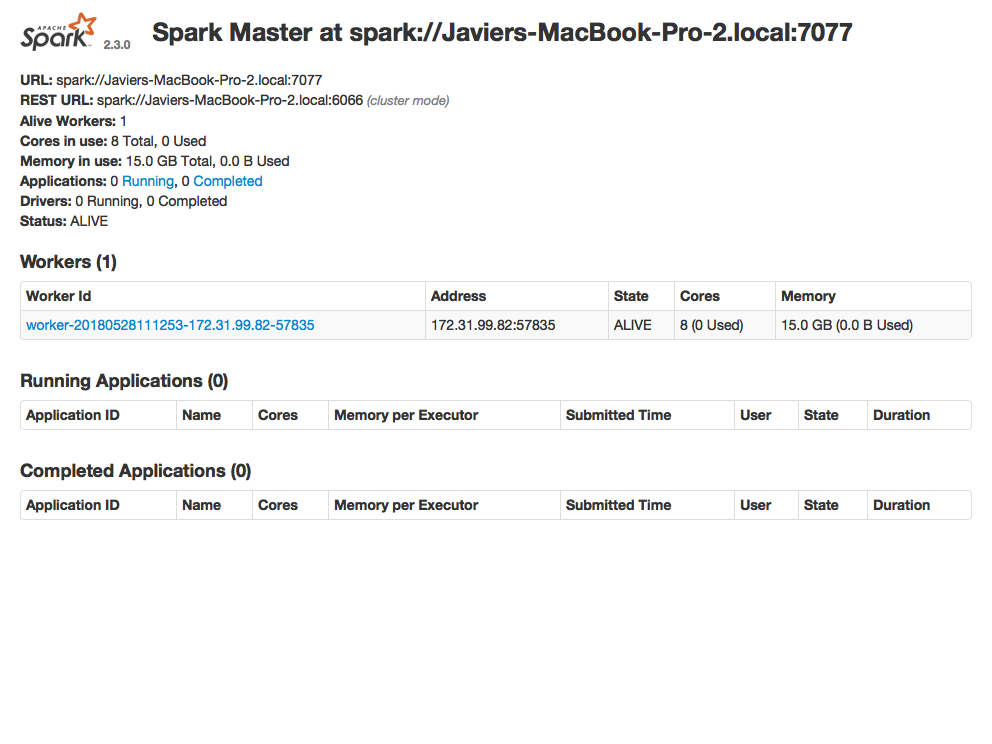
\includegraphics[width=13.78in]{images/05-clusters-spark-standalone-web-ui} 

}

\caption{Spark Standalone Web Interface.}\label{fig:spark-standalone-web-ui}
\end{figure}

Notice that there is one worker register in Spark standalone, you can
follow the link to this worker node to see additional information:

\begin{figure}

{\centering 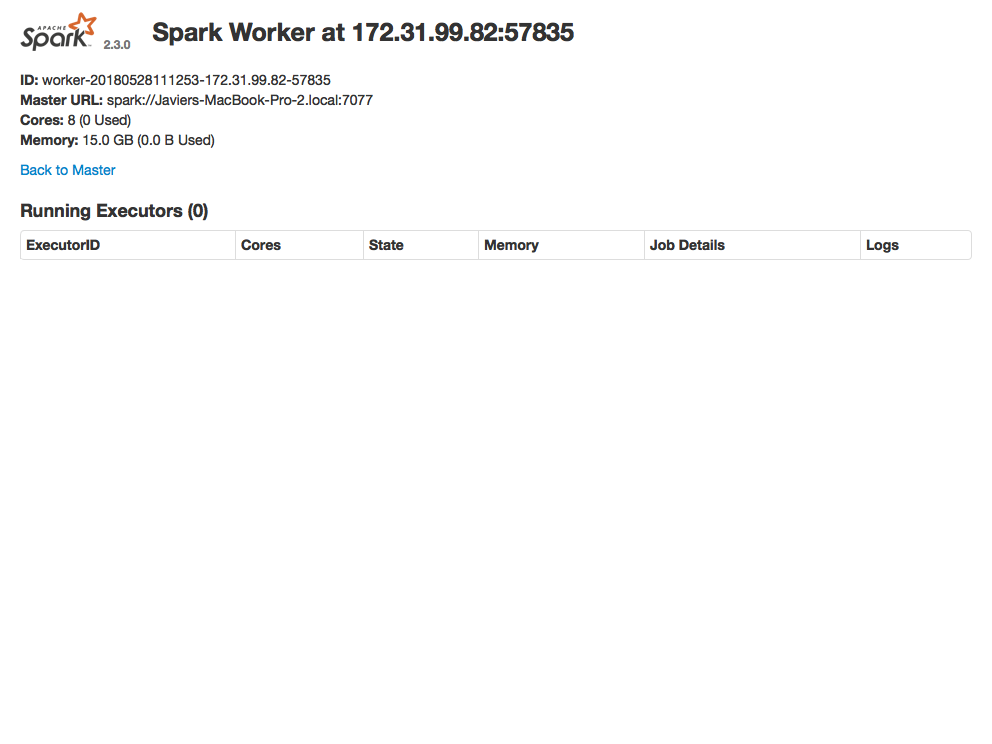
\includegraphics[width=13.78in]{images/05-clusters-spark-standalone-web-ui-worker} 

}

\caption{Spark Standalone Worker Web Interface.}\label{fig:spark-standalone-web-ui-worker}
\end{figure}

Once data analysis is complete, one can simply stop all the running
nodes in this local cluster by running:

\begin{Shaded}
\begin{Highlighting}[]
\NormalTok{stop_all <-}\StringTok{ }\KeywordTok{file.path}\NormalTok{(spark_home, }\StringTok{"sbin"}\NormalTok{, }\StringTok{"stop-all.sh"}\NormalTok{)}
\KeywordTok{system2}\NormalTok{(stop_all)}
\end{Highlighting}
\end{Shaded}

A similar approach can be followed to configure a cluster by running
each \texttt{start-slave.sh} command over each machine in the cluster.

Further reading:
\href{https://spark.apache.org/docs/latest/spark-standalone.html}{Spark
Standalone Mode}

\hypertarget{yarn}{%
\subsection{Yarn}\label{yarn}}

YARN for short, or Hadoop YARN, is the resource manager introduced in
2012 to the Hadoop project. As mentioned in in the
\protect\hyperlink{intro}{Introduction} chapter, Spark was built
initially to speed up computation over Hadoop; then, when Hadoop 2 was
launched, it introduced YARN as a component to manage resources in the
cluster, to this date, using Hadoop YARN with Apache Spark is still very
common.

YARN applications can be submitted in two modes: \textbf{yarn-client}
and \textbf{yarn-cluster}. In yarn-cluster mode the driver is running
remotely, while in yarn-client mode, the driver is on the machine that
started the job, \texttt{sparklyr} supports both modes.

\begin{figure}

{\centering 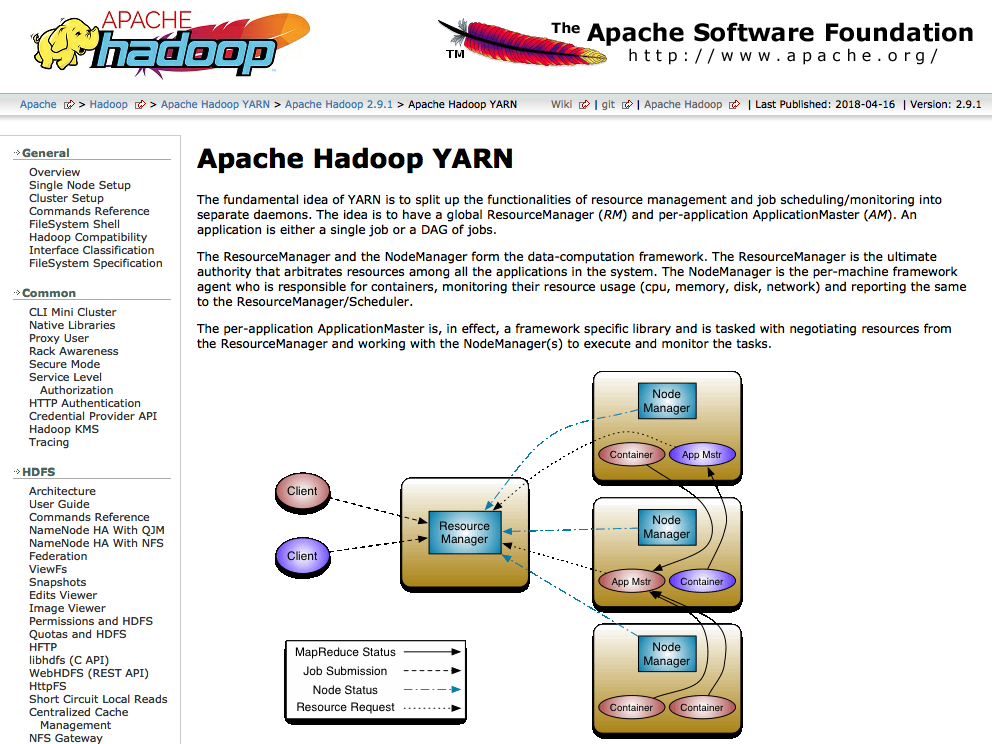
\includegraphics[width=13.78in]{images/05-clusters-yarn} 

}

\caption{Hadoop YARN Site}\label{fig:hadoop-yarn}
\end{figure}

Further reading:
\href{https://spark.apache.org/docs/latest/running-on-yarn.html}{Running
Spark on YARN}

\hypertarget{mesos}{%
\subsection{Mesos}\label{mesos}}

Apache Mesos is an open-source project to manage computer clusters.
Mesos began as a research project in the UC Berkeley RAD Lab by then PhD
students Benjamin Hindman, Andy Konwinski, and Matei Zaharia, as well as
professor Ion Stoica. Mesos uses Linux
\href{https://en.wikipedia.org/wiki/Cgroups}{Cgroups} to provide
isolation for CPU, memory, I/O and file system.

\begin{figure}

{\centering 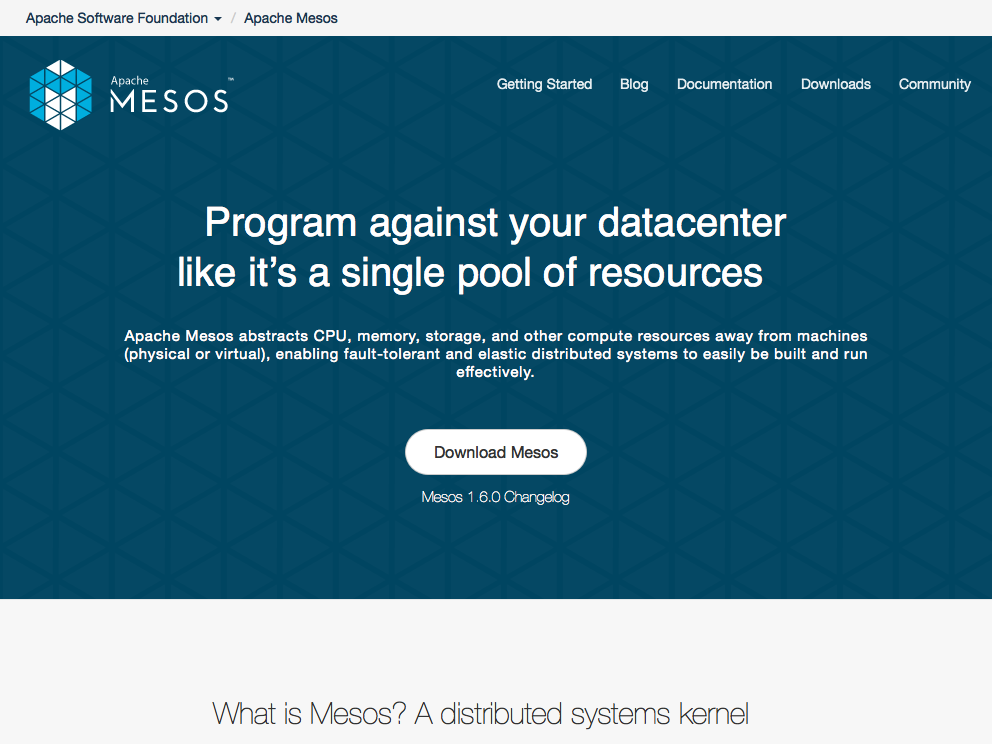
\includegraphics[width=13.78in]{images/05-clusters-mesos} 

}

\caption{Mesos Landing Site}\label{fig:mesos-spark}
\end{figure}

Further reading:
\href{https://spark.apache.org/docs/latest/running-on-mesos.html}{Running
Spark on Mesos}

\hypertarget{kubernetes}{%
\subsection{Kubernetes}\label{kubernetes}}

Kubernetes is an open-source container-orchestration system for
automating deployment, scaling and management of containerized
applications that was originally designed by Google and now maintained
by the \href{https://www.cncf.io/}{Cloud Native Computing Foundation}.

\begin{figure}

{\centering 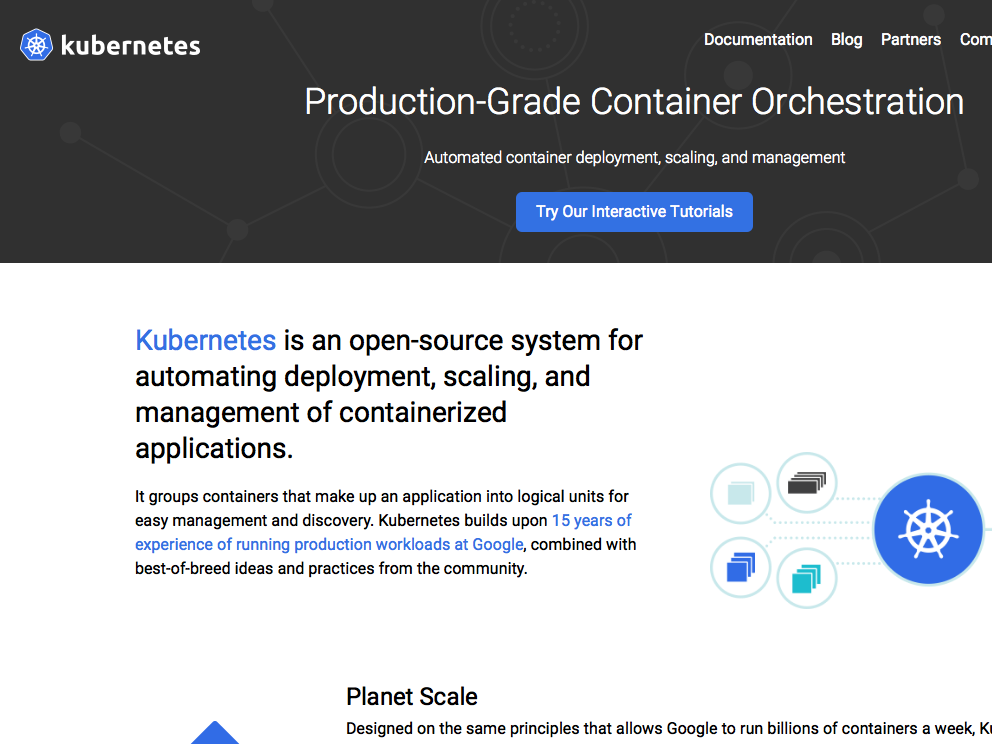
\includegraphics[width=13.78in]{images/05-clusters-kubernetes} 

}

\caption{Kubernetes Landing Site.}\label{fig:kubernetes-spark}
\end{figure}

Further reading:
\href{https://spark.apache.org/docs/latest/running-on-kubernetes.html}{Running
Spark on Kubernetes}

\hypertarget{on-premise}{%
\section{On-Premise}\label{on-premise}}

As mentioned in the overview section, on-premise clusters represent a
set of computing instances procured, colocated and managed by staff
members from your organization. These clusters can be highly customized
and controlled; however, they can also inccur significant initial
expenses and maintenance costs.

One can use a cluster manager in on-premise clusters as described in the
previous section; however, many organizations choose to partner with
companies providing additional management software, services and
resources to manage software in their cluster including, but not limited
to, Apache Spark. Some of the on-premise cluster providers include:
Cloudera, Hortonworks and MapR to mention a few which will be briefly
introduced.

\hypertarget{cloudera}{%
\subsection{Cloudera}\label{cloudera}}

Cloudera, Inc.~is a United States-based software company that provides
Apache Hadoop and Apache Spark-based software, support and services, and
training to business customers.

Cloudera's hybrid open-source Apache Hadoop distribution, CDH (Cloudera
Distribution Including Apache Hadoop), targets enterprise-class
deployments of that technology. Cloudera says that more than 50\% of its
engineering output is donated upstream to the various Apache-licensed
open source projects (Apache Hive, Apache Avro, Apache HBase, and so on)
that combine to form the Apache Hadoop platform. Cloudera is also a
sponsor of the Apache Software Foundation.

\begin{figure}

{\centering 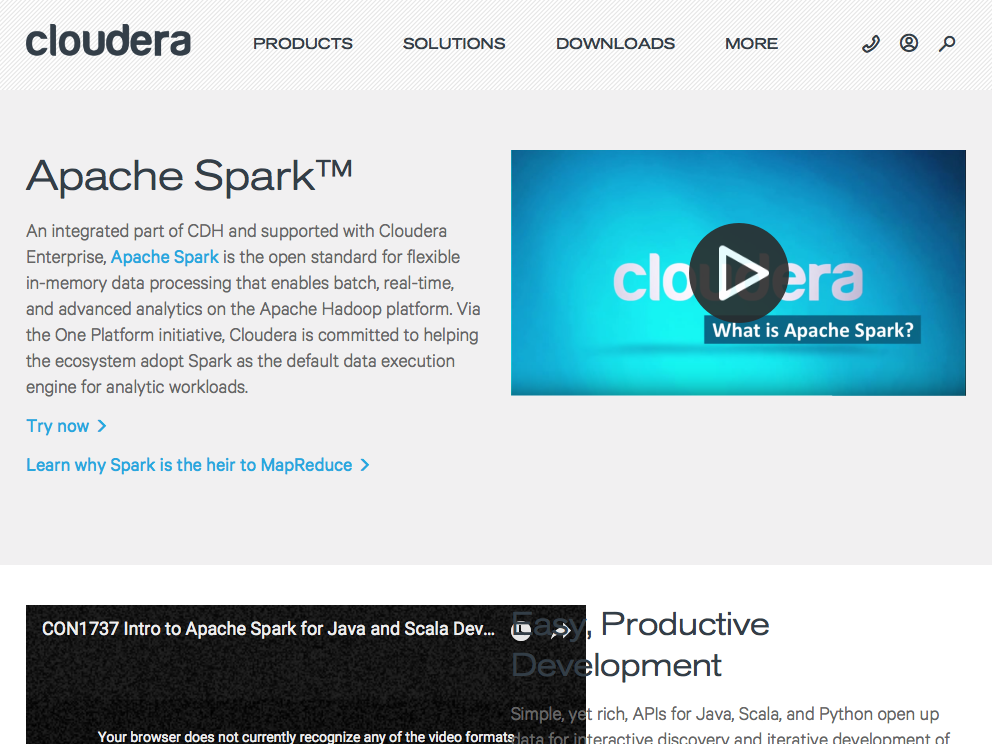
\includegraphics[width=13.78in]{images/05-clusters-cloudera} 

}

\caption{Cloudera Landing Site.}\label{fig:cloudera-spark}
\end{figure}

\hypertarget{hortonworks}{%
\subsection{Hortonworks}\label{hortonworks}}

Hortonworks is a big data software company based in Santa Clara,
California. The company develops, supports, and provides expertise on an
expansive set of entirely open source software designed to manage data
and processing for everything from IOT, to advanced analytics and
machine learning. Hortonworks believes it is a data management company
bridging the cloud and the datacenter.

\begin{figure}

{\centering 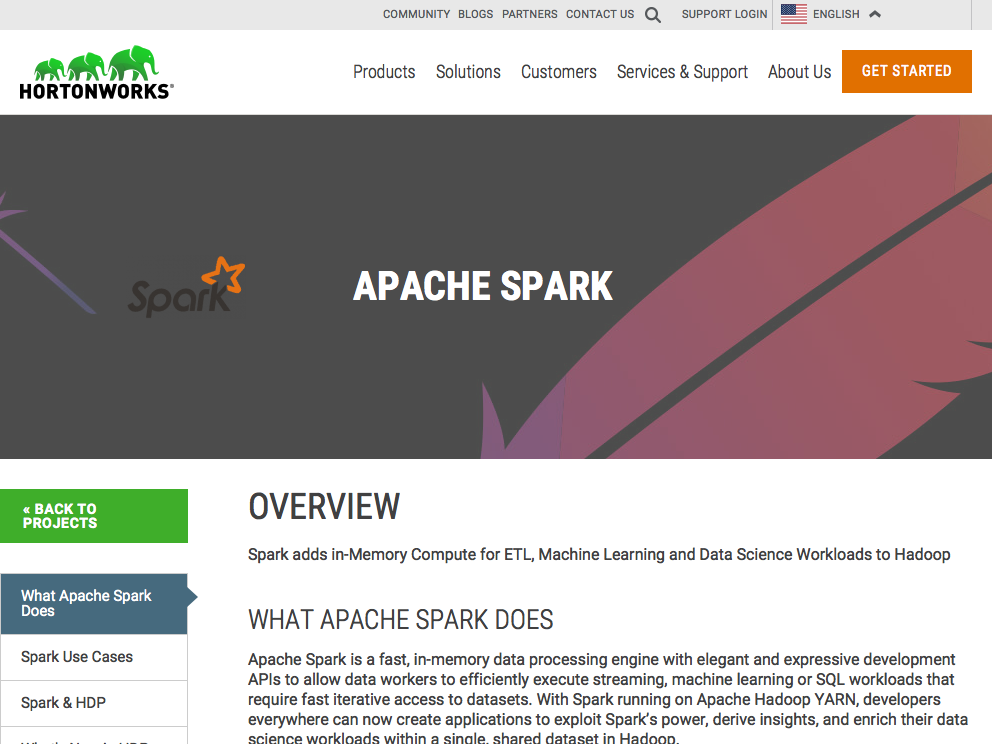
\includegraphics[width=13.78in]{images/05-clusters-hortonworks} 

}

\caption{Hortonworks Landing Site.}\label{fig:hortonworks-spark}
\end{figure}

\hypertarget{mapr}{%
\subsection{MapR}\label{mapr}}

MapR is a business software company headquartered in Santa Clara,
California. MapR provides access to a variety of data sources from a
single computer cluster, including big data workloads such as Apache
Hadoop and Apache Spark, a distributed file system, a multi-model
database management system, and event stream processing, combining
analytics in real-time with operational applications. Its technology
runs on both commodity hardware and public cloud computing services.

\begin{figure}

{\centering 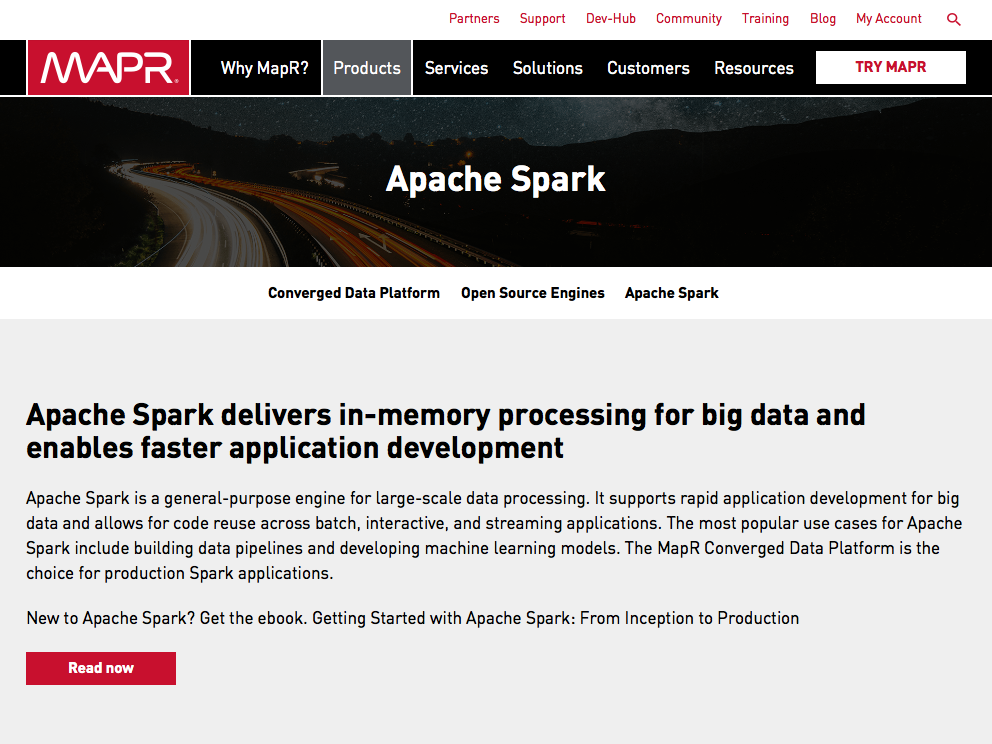
\includegraphics[width=13.78in]{images/05-clusters-mapr} 

}

\caption{MapR Landing Site.}\label{fig:mapr-spark}
\end{figure}

\hypertarget{cloud}{%
\section{Cloud}\label{cloud}}

For those readers that don't have a cluster yet, it is likely that you
will want to choose a cloud cluster, this section will briefly mention
some of the major cloud infrastructure providers as a starting point to
choose the right one for you.

It is worth mentioning that in a cloud service model, the compute
instances are charged by the hour and times the number of instances
reserved for your cluster. Since the cluster size is flexible, it is a
good practice to start with small clusters and scale compute resources
as needed. Even if you know in advance that a cluster of significant
size will be required, starting small provides an opportunity to
troubleshoot issues at a lower cost since it's unlikely that your data
analysis will run at scale flawlessly on the first try.

The major providers of cloud computing infrastructure are: Amazon,
Google and Microsoft that this section will briefly introduce.

\hypertarget{amazon}{%
\subsection{Amazon}\label{amazon}}

Amazon provides cloud services through
\href{https://aws.amazon.com/}{Amazon Web Services}; more specifically,
they provide an on-demand Spark cluster through
\href{https://aws.amazon.com/emr/}{Amazon Elastic Map Reduce} or EMR for
short.

\begin{figure}

{\centering 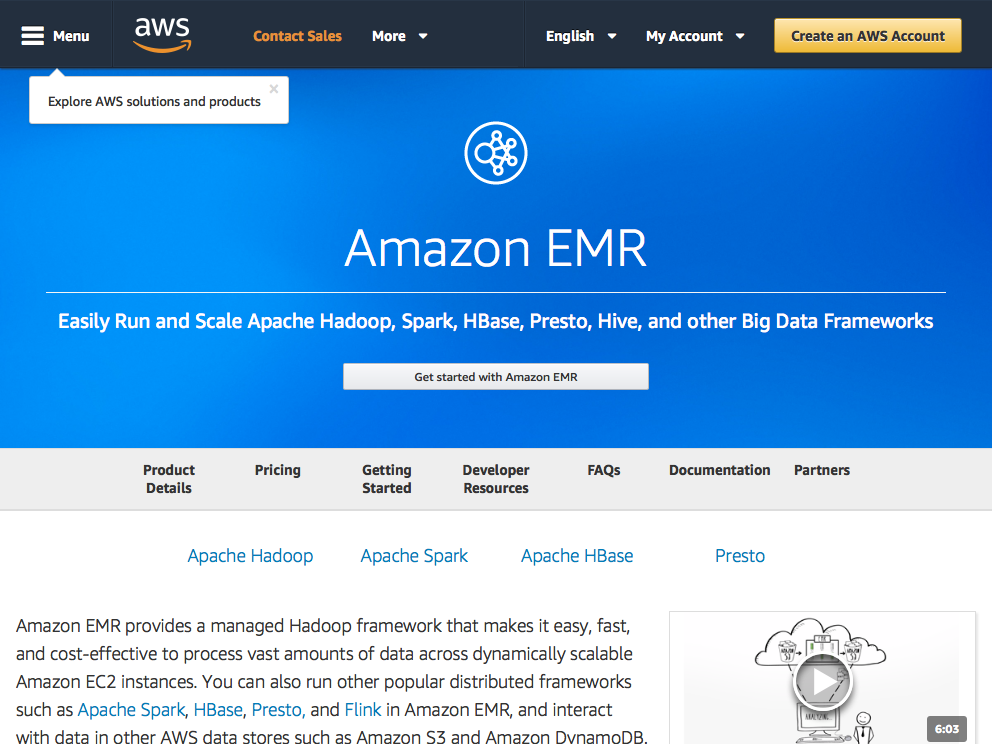
\includegraphics[width=13.78in]{images/05-clusters-amazon-emr} 

}

\caption{Amazon EMR Landing Site.}\label{fig:amazon-emr}
\end{figure}

\hypertarget{google}{%
\subsection{Google}\label{google}}

Google provides their on-demand computing services through their
\href{https://cloud.google.com/}{Google Cloud}, on-demand Spark cluster
are provided by \href{https://cloud.google.com/dataproc/}{Google
Dataproc}.

\begin{figure}

{\centering 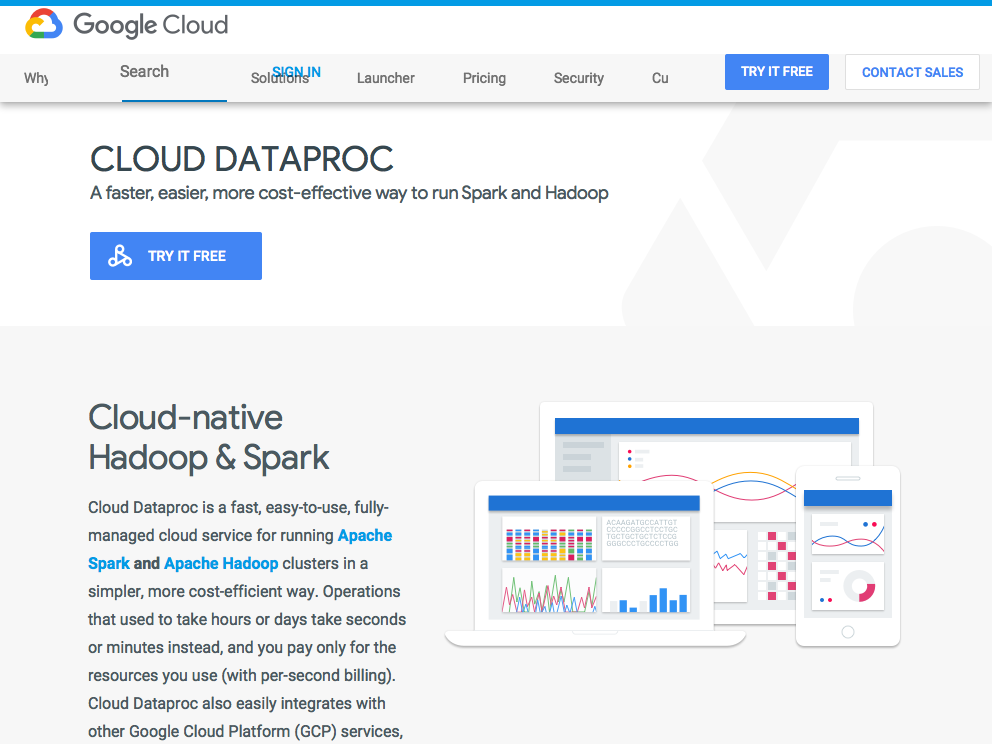
\includegraphics[width=13.78in]{images/05-clusters-dataproc} 

}

\caption{Google Dataprox Landing Site.}\label{fig:google-dataproc}
\end{figure}

\hypertarget{microsoft}{%
\subsection{Microsoft}\label{microsoft}}

Microsoft provides cloud services thorugh
\href{https://azure.microsoft.com/}{Microsft Azure} and Spark clusters
through
\href{https://azure.microsoft.com/en-us/services/hdinsight/}{Azure
HDInsight}.

\begin{figure}

{\centering 
\includegraphics[width=13.78in]{images/05-clusters-azure} 

}

\caption{Azure HDInsight Landing Site.}\label{fig:azure-hdinsight}
\end{figure}

\hypertarget{tools}{%
\section{Tools}\label{tools}}

While using only R and Spark can be sufficient for some clusters, it is
common to install complementary tools in your cluster to improve:
monitoring, sql analysis, workflow coordination, etc. with applications
like \href{http://ganglia.info/}{Ganglia},
\href{http://gethue.com/}{Hue} and
\href{https://oozie.apache.org}{Oozie} respectevly. This secton is not
meant to cover all, but rather mention two that are relevant to R and
\texttt{sparklyr}.

\hypertarget{rstudio}{%
\subsection{RStudio}\label{rstudio}}

RStudio's open source and professional products, like: RStudio Server,
\href{https://www.rstudio.com/products/rstudio-server-pro/}{RStudio
Server Pro}, \href{https://www.rstudio.com/products/shiny/}{Shiny
Server}, \href{https://www.rstudio.com/products/shiny-server-pro/}{Shiny
Server Pro}, or \href{https://www.rstudio.com/products/connect/}{RStudio
Connect}; can be installed within the cluster to support many R
workflows, while \texttt{sparklyr} does not require any additional
tools, they provide significant productivity gains worth considering.

\begin{figure}

{\centering 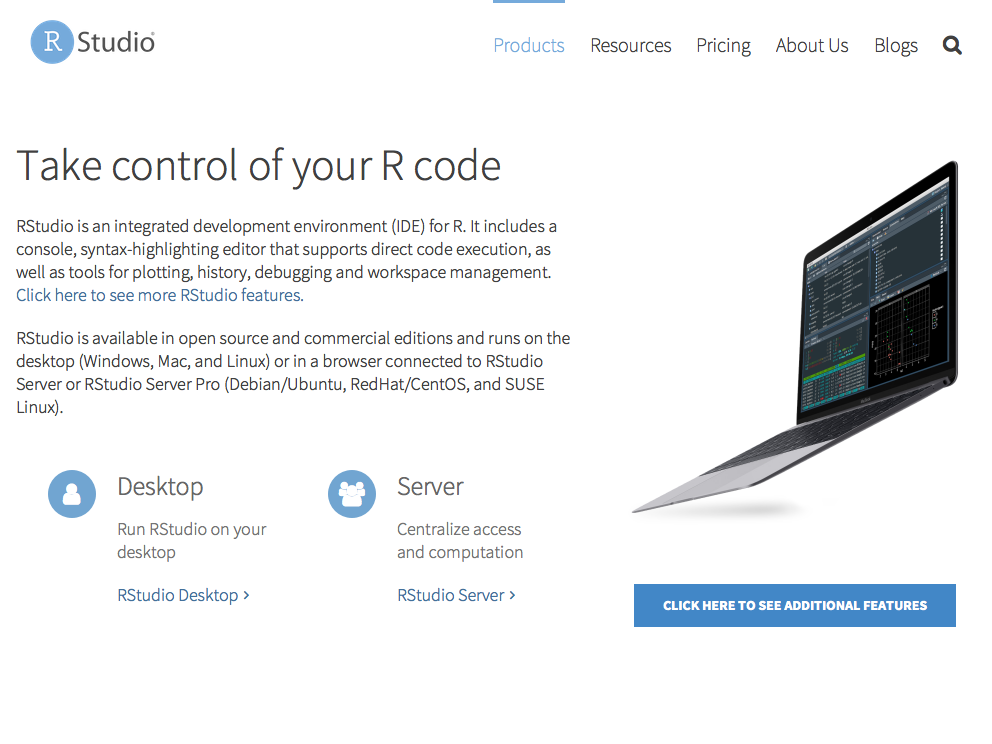
\includegraphics[width=13.78in]{images/05-clusters-rstudio-server} 

}

\caption{Rstudio Server}\label{fig:rstudio-server}
\end{figure}

\hypertarget{clusters-livy}{%
\subsection{Livy}\label{clusters-livy}}

\href{https://livy.incubator.apache.org/}{Apapche Livy} is an incubation
project in Apache providing support to use Spark clusters remotely
through a web interface. It is ideal to connect directly into the Spark
cluster; however, there are times where connecting directly to the
cluster is not feasible. When facing those constraints, one can consider
installing Livy in their cluster and secure it properly to enable remote
use over web protocols.

However, there is a significant performance overhead from using Livy in
\texttt{sparklyr} for experimentation, meaning that, executing many
client comamnds over Livy has a significant overhead; however, running a
few commands to generate complex analysis is usually performant since
the performance overhead of starting computation can be insignificant
compared to the actual cluster computation.

\begin{figure}

{\centering 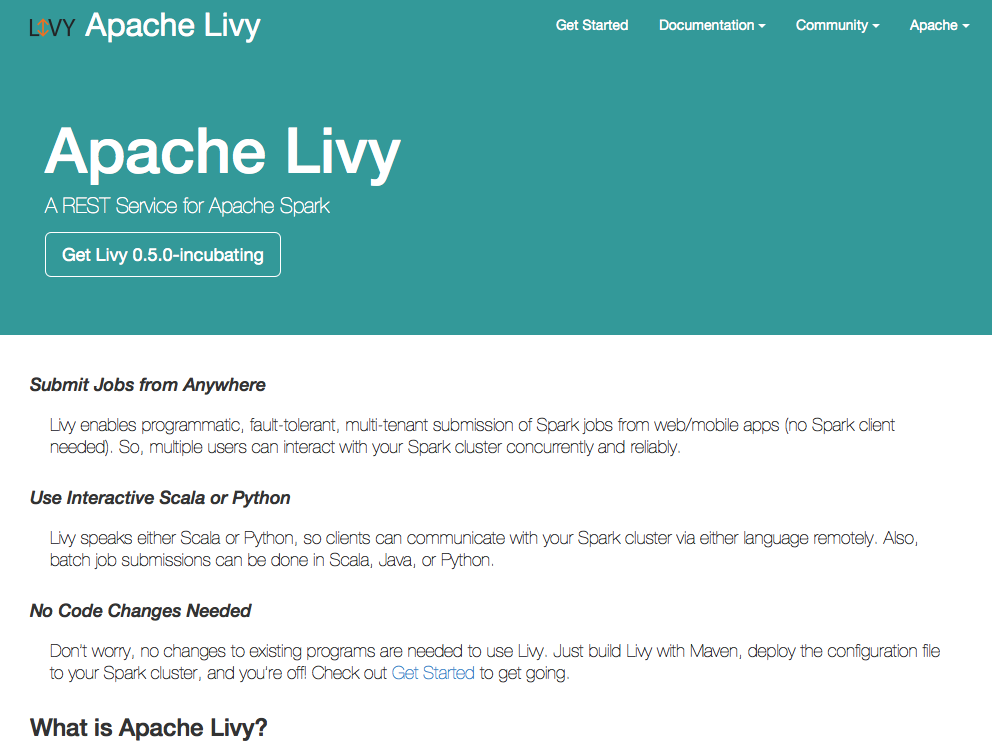
\includegraphics[width=13.78in]{images/05-clusters-apache-livy} 

}

\caption{Apache Livy Landing Site.}\label{fig:apache-livy}
\end{figure}

To help test Livy locally, \texttt{sparklyr} provides support to list,
install, start and stop a local Livy instance by executing:

\begin{Shaded}
\begin{Highlighting}[]
\CommentTok{# List versions of Livy available to install}
\KeywordTok{livy_available_versions}\NormalTok{()}
\end{Highlighting}
\end{Shaded}

\begin{verbatim}
##    livy
## 1 0.2.0
## 2 0.3.0
## 3 0.4.0
## 4 0.5.0
\end{verbatim}

\begin{Shaded}
\begin{Highlighting}[]
\CommentTok{# Install default Livy version}
\KeywordTok{livy_install}\NormalTok{()}

\CommentTok{# List installed Livy services}
\KeywordTok{livy_installed_versions}\NormalTok{()}

\CommentTok{# Start the Livy service}
\KeywordTok{livy_service_start}\NormalTok{()}

\CommentTok{# Stops the Livy service}
\KeywordTok{livy_service_stop}\NormalTok{()}
\end{Highlighting}
\end{Shaded}

The default address for this local Livy service is
\url{http://localhost:8998}

\hypertarget{recap-1}{%
\section{Recap}\label{recap-1}}

This chapter explained the history and tradeoffs of on-premise, cloud
computing and presented Kubernetes as a promising framework to provide
flexibility across on-premise and cloud providers. It also introduced
cluster managers (Spark Standalone, YARN, Mesos and Kubernetes) as the
software needed to run Spark as a cluster application. This chapter
briefly mentioned on-premise cluster providers like Cloudera,
Hortonworks and MapR as well as the major cloud providers: Amazon,
Google and Microsoft.

While this chapter provided a solid foundation to understand current
computing trends, cluster tools and providers useful to perform data
science; it falls short to help those tasked with deliberately choosing
a cluster manager, service provider or architecture. If you have this
task assigned to you, use this chapter as a starting point to reach to
many more resources to complete your understanding of the platform your
organization needs.

The next chapter, \protect\hyperlink{connections-1}{Connections},
assumes a Spark cluster is already available to you and will focus on
understanding how to connect to it from sparklyr.

\hypertarget{connections}{%
\chapter{Connections}\label{connections}}

The previous chapter, \protect\hyperlink{clusters}{Clusters}, presented
the major cluster computing paradigms, cluster managers and cluster
providers; this section explains the internal components of a Spark
cluster and the how to perform connections to any cluster running Apache
Spark.

\hypertarget{overview-2}{%
\section{Overview}\label{overview-2}}

Before explaining how to connect to Spark clusters, it is worth
discussing the components of a Spark cluster and how they interact, this
is often known as the cluster architecture of Apache Spark.

First, lets go over a couple definitions. As you know form previous
chapters, a cluster is a collection of machines to perform analysis
beyond a single computer. However, in distributed systems and clusters
literature, we often reffer to each physical machine as a compute
instance, compute node, or simply instance or node for short. It is
helpful to remind this while reading through this chapter and making use
of external resource.

In a Spark cluster, there are three types of compute instances that are
relevant to Spark: The \textbf{driver node}, the \textbf{worker nodes}
and the \textbf{cluster manager}. A cluster manager is a service that
allos Spark to be executed in the clsuter and was explained in the
\href{Managers}{Cluster Managers} section. The driver node is tasked
with delegating work to the worker nodes, but also for aggregating their
results and iterating further if needed. For the most part, aggregation
happens in the worker nodes; however, even after the nodes aggregate
data, it is often the case that the driver node would have to aggregate
the worker results. Therefore, the driver node has at least, but often,
much more compute resources (read RAM, CPU, Local Storage, etc.) then
the worker node.

Strictly speaking, the driver node and worker nodes are just names
assigned to machines with particular roles, while the actual computation
in the driver node is performed by the \textbf{spark context}. The Spark
context is a Spark component tasked with scheduling tasks, managing data
and so on. In the worker nodes, the actual computation is performed
under a \textbf{spark executor}, which is also a Spark component tasked
with executing subtasks against a data partition.

\begin{figure}

{\centering 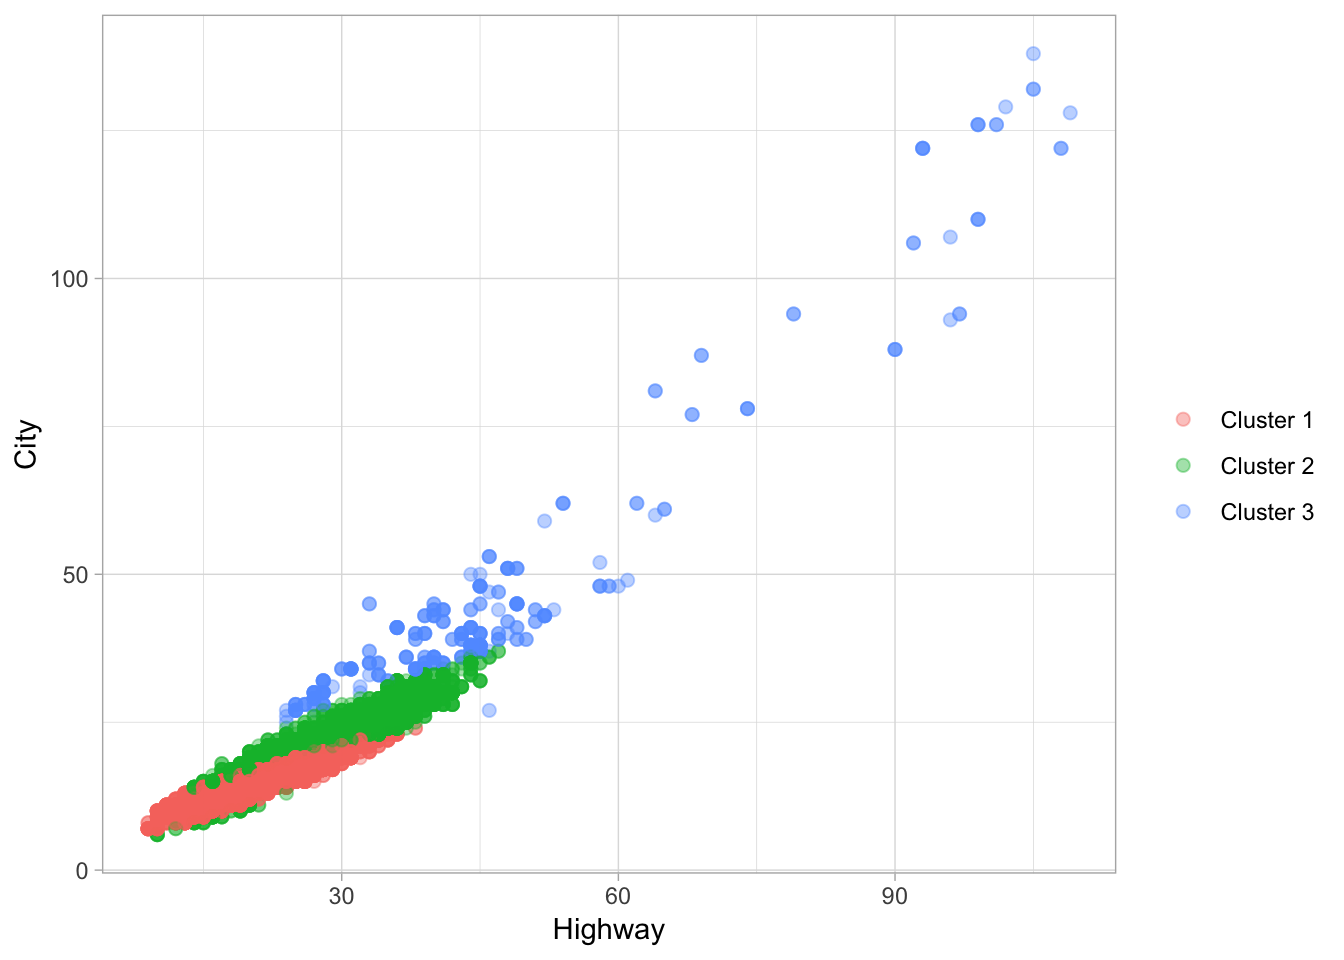
\includegraphics[width=1\linewidth,height=220pt]{the-r-in-spark_files/figure-latex/unnamed-chunk-29-1} 

}

\caption{Apache Spark Architecture}\label{fig:unnamed-chunk-29}
\end{figure}

If you already have an Spark cluster in their organization, you should
ask your cluster administrator to provide connection information for
this cluster and read carefully their usage policies and constraints. A
cluster is usually shared among many users so you want to be respectful
of others time and resources while using a shared cluster environment.
Your system administrator will describe if it's an \textbf{on-premise}
vs \textbf{cloud} cluster, the \textbf{cluster manager} being used,
supported \textbf{connections} and supported \textbf{tools}. You can use
this information to jump directly to \protect\hyperlink{local}{Local},
\protect\hyperlink{standalone}{Standalone},
\protect\hyperlink{yarn-1}{Yarn}, \protect\hyperlink{mesos-1}{Mesos},
\protect\hyperlink{livy}{Livy} or
\protect\hyperlink{kubernetes-1}{Kubernetes} based on the information
provided to you.

\hypertarget{edge-nodes}{%
\subsection{Edge Nodes}\label{edge-nodes}}

Before connecting to Apache Spark, you will first have to connect to the
cluster. Usually, by connecting to an edge node within the cluster. An
edge node, is a machine that can accessed from outside the cluster but
which is also part of the cluster. There are two methods to connect to
this edge instance:

\begin{itemize}
\tightlist
\item
  \textbf{Terminal}: Using a
  \href{https://en.wikipedia.org/wiki/Computer_terminal}{computer
  terminal} applicaiton, one can use a
  \href{https://en.wikipedia.org/wiki/Secure_Shell}{secure shell} to
  establish a remote connection into the cluster, once you connect into
  the cluster, you can launch R and then use \texttt{sparklyr}.
\item
  \textbf{Web Browser}: While using \texttt{sparklyr} from a terminal is
  possible, it is usually more producty to install a \textbf{web server}
  in an edge node that provides more tools and functionality to run R
  with \texttt{sparklyr}. Most likely, you will want to consider using
  \href{RStudio\%20Server}{RStudio Server} rather than connecting from
  the terminal.
\end{itemize}

\begin{figure}

{\centering \includegraphics[width=1\linewidth,height=140pt]{the-r-in-spark_files/figure-latex/unnamed-chunk-30-1} 

}

\caption{Using a Spark Cluster from an Edge Node}\label{fig:unnamed-chunk-30}
\end{figure}

\hypertarget{spark-home}{%
\subsection{Spark Home}\label{spark-home}}

It is important to mention that, while connecting to a Spark cluster,
you will need to find out the correct \texttt{SPARK\_HOME} path which
contains the installation of Spark in the given instance. The
\texttt{SPARK\_HOME} path must be set as an environment variable before
connecting or explicitly specified in \texttt{spark\_connect()} using
the \texttt{spark\_home} parameter.

For system administrators, we recommend you set \texttt{SPARK\_HOME} for
all the users in your cluster; however, if this is not set in your
cluster you can also specify \texttt{SPARK\_HOME} while using
\texttt{spark\_connect()} as follows:

\begin{Shaded}
\begin{Highlighting}[]
\NormalTok{sc <-}\StringTok{ }\KeywordTok{spark_connect}\NormalTok{(}\DataTypeTok{master =} \StringTok{"cluster-master"}\NormalTok{, }\DataTypeTok{spark_home =} \StringTok{"local/path/to/spark"}\NormalTok{)}
\end{Highlighting}
\end{Shaded}

Where \texttt{cluster-master} is set to the correct cluster manager
master for \href{Standalone}{Spark Standalone}, \href{Yarn}{YARN},
\protect\hyperlink{mesos-1}{Mesos}, etc.

\hypertarget{types}{%
\section{Types}\label{types}}

\hypertarget{local}{%
\subsection{Local}\label{local}}

When connecting to Spark in local mode, Spark starts as a single
application simulating a cluster with a single node, this is not a
proper computing cluster but is ideal to perform work offline and
troubleshoot issues. A local connection to Spark is represented in the
following diagram:

\begin{figure}

{\centering \includegraphics[width=1\linewidth,height=160pt]{the-r-in-spark_files/figure-latex/unnamed-chunk-32-1} 

}

\caption{Local Connection Diagram}\label{fig:unnamed-chunk-32}
\end{figure}

Notice that in the local connections diagram, there is no cluster
manager nor worker process since, in local mode, everything runs inside
the driver application. It's also worth pointing out that
\texttt{sparklyr} starts the Spark Context through
\texttt{spark-submit}, a script available in every Spark installation to
enable users to submit custom application to Spark which
\texttt{sparklyr} makes use of to submit itself to Spark. For the
curious reader, the \protect\hyperlink{contributing}{Contributing}
chapter explains the internal processes that take place in
\texttt{sparklyr} to submit this application and connect properly from
R.

To perform this local connection, we can connect with the following
familiar code used in previous chapters:

\begin{Shaded}
\begin{Highlighting}[]
\CommentTok{# Connect to local Spark instance}
\NormalTok{sc <-}\StringTok{ }\KeywordTok{spark_connect}\NormalTok{(}\DataTypeTok{master =} \StringTok{"local"}\NormalTok{)}
\end{Highlighting}
\end{Shaded}

By default, \texttt{sparklyr}, will connect using as many CPU cores are
available in your compute instance; however, this can be customized by
connecting using \texttt{master="local{[}n{]}"}, where \texttt{n} is the
desired number of cores to use. For example, we can connect using only 2
CPU cores as follows:

\begin{Shaded}
\begin{Highlighting}[]
\CommentTok{# Connect to local Spark instance using 2 cores}
\NormalTok{sc <-}\StringTok{ }\KeywordTok{spark_connect}\NormalTok{(}\DataTypeTok{master =} \StringTok{"local[2]"}\NormalTok{)}
\end{Highlighting}
\end{Shaded}

\hypertarget{standalone}{%
\subsection{Standalone}\label{standalone}}

Connecting to a Spark Standalone cluster requires the location of the
cluster manager's master instance, this location can be found in the
cluster manager web interface as described in the
\href{standalone\%20cluster}{clusters-standalone} section, you can find
this location by looking for a URL starting with \texttt{spark://}.

A connection in standalone mode starts from \texttt{sparklyr} launching
\texttt{spark-submit} to submit the \texttt{sparklyr} application and
creating the Spark Context, which requests executors to Spark's
standalone cluster manager in the \texttt{master} location:

\begin{figure}

{\centering \includegraphics[width=1\linewidth]{the-r-in-spark_files/figure-latex/unnamed-chunk-35-1} 

}

\caption{Spark Standalone Connection Diagram}\label{fig:unnamed-chunk-35}
\end{figure}

In order to connect, use \texttt{master="spark://hostname:port"} in
\texttt{spark\_connect()} as follows:

\begin{Shaded}
\begin{Highlighting}[]
\NormalTok{sc <-}\StringTok{ }\KeywordTok{spark_connect}\NormalTok{(}\DataTypeTok{master =} \StringTok{"spark://hostname:port"}\NormalTok{)}
\end{Highlighting}
\end{Shaded}

\hypertarget{yarn-1}{%
\subsection{Yarn}\label{yarn-1}}

Hadoop YARN supports two connection modes: YARN Client and YARN Cluster.
However, YARN Client mode is much more common that YARN Cluster since
it's more efficient and easier to set up.

\hypertarget{yarn-client}{%
\subsubsection{Yarn Client}\label{yarn-client}}

When connecting in YARN Client mode, the driver instance runs R,
sparklyr and the Spark Context which requests worker nodes from YARN to
run Spark executors as follows:

\begin{figure}

{\centering \includegraphics[width=1\linewidth]{the-r-in-spark_files/figure-latex/unnamed-chunk-37-1} 

}

\caption{YARN Client Connection Diagram}\label{fig:unnamed-chunk-37}
\end{figure}

To connect, one can simply run with \texttt{master\ =\ "yarn"} as
follows:

\begin{Shaded}
\begin{Highlighting}[]
\NormalTok{sc <-}\StringTok{ }\KeywordTok{spark_connect}\NormalTok{(}\DataTypeTok{master =} \StringTok{"yarn-client"}\NormalTok{)}
\end{Highlighting}
\end{Shaded}

Once connected, you can use all techniques described in previous
chapters using the \texttt{sc} connection; for instances, you can do
\href{analysis}{data analysis} or
\protect\hyperlink{modeling}{modeling}.

\hypertarget{yarn-cluster}{%
\subsubsection{Yarn Cluster}\label{yarn-cluster}}

The main difference between YARN Cluster mode and YARN Client mode is
that in YARN Cluster mode, the driver node is not required to be the
node where R and sparklyr get started; instead, the driver node remains
the designated driver node which is usually a different node than the
edge node where R is running. It can be helpful to consider using YARN
Cluster when the edge node has too many concurrent users, is lacking
computing resources or where tools (like RStudio) need to be managed
independently of other clsuter resources.

\begin{figure}

{\centering \includegraphics[width=1\linewidth]{the-r-in-spark_files/figure-latex/unnamed-chunk-39-1} 

}

\caption{YARN Cluster Connection Diagram}\label{fig:unnamed-chunk-39}
\end{figure}

To connect in YARN Cluster mode, we can simple run:

\begin{Shaded}
\begin{Highlighting}[]
\NormalTok{sc <-}\StringTok{ }\KeywordTok{spark_connect}\NormalTok{(}\DataTypeTok{master =} \StringTok{"yarn-cluster"}\NormalTok{)}
\end{Highlighting}
\end{Shaded}

This connection assumes that the node running \texttt{spark\_connect()}
is properly configured, meaning that, \texttt{yarn-site.xml} exists and
the \texttt{YARN\_CONF\_DIR} environment variable is properly set. When
using Hadoop as a file system, one would also need the
\texttt{HADOOP\_CONF\_DIR} environment variable properly configured.
This configuration is usually provided by your system administrator and
is not something that you would have to manually configure.

\hypertarget{livy}{%
\subsection{Livy}\label{livy}}

As opposed to other connection methods which require using an edge node
in the cluster, \href{clusters-livy}{Livy} Livy provides a \textbf{Web
API} that makes the Spark cluster accessible from outside the cluster
and neither requires a local installation in the client. Once connected
through the Web API, the \textbf{Livy Service} starts the Spark context
by requesting reosurces from the cluster manager and distributing work
as usual.

\begin{figure}

{\centering \includegraphics[width=1\linewidth]{the-r-in-spark_files/figure-latex/unnamed-chunk-41-1} 

}

\caption{Livy Connection Diagram}\label{fig:unnamed-chunk-41}
\end{figure}

Conencting through Livy requires the URL to the Livy service which
should be similar to \texttt{https://hostname:port/livy}. Since remote
connections are allowed, connections usually requires, at the very
least, basic authentication:

\begin{Shaded}
\begin{Highlighting}[]
\NormalTok{sc <-}\StringTok{ }\KeywordTok{spark_connect}\NormalTok{(}\DataTypeTok{master =} \StringTok{"https://hostname:port/livy"}\NormalTok{, }\DataTypeTok{method =} \StringTok{"livy"}\NormalTok{, }\DataTypeTok{config =} \KeywordTok{livy_config}\NormalTok{(}
  \DataTypeTok{username=}\StringTok{"<username>"}\NormalTok{,}
  \DataTypeTok{password=}\StringTok{"<password>"}
\NormalTok{))}
\end{Highlighting}
\end{Shaded}

Once connected through Livy, operations you can make use of an other
\texttt{sparklyr} feature; however, Livy is not suitable for
experimental data analysis, since executing commands have a significant
delay; that said, while running long running computations, this overhead
could be considered irrelevant. In general, it is preffered to avoid
using Livy and work directly within an edge node in the cluster; if this
is not feasible, using Livy could be a reasonable approach.

\hypertarget{mesos-1}{%
\subsection{Mesos}\label{mesos-1}}

Similar to YARN, Mesos supports client mode and a cluster mode. However,
\texttt{sparklyr} currently only supports client mode for Mesos.

\begin{figure}

{\centering \includegraphics[width=1\linewidth]{the-r-in-spark_files/figure-latex/unnamed-chunk-43-1} 

}

\caption{Mesos Connection Diagram}\label{fig:unnamed-chunk-43}
\end{figure}

Connecting requires the address to the Mesos master node, usually in the
form of \texttt{mesos://host:port} or
\texttt{mesos://zk://host1:2181,host2:2181,host3:2181/mesos} for Mesos
using ZooKeeper.

\begin{Shaded}
\begin{Highlighting}[]
\NormalTok{sc <-}\StringTok{ }\KeywordTok{spark_connect}\NormalTok{(}\DataTypeTok{master =} \StringTok{"mesos://host:port"}\NormalTok{)}
\end{Highlighting}
\end{Shaded}

\hypertarget{kubernetes-1}{%
\subsection{Kubernetes}\label{kubernetes-1}}

Kubernetes cluster do not support client modes similar to Mesos or YARN,
instead, the connection model is similar to YARN Cluster, where the
driver node is assigned by Kubernetes.

\begin{figure}

{\centering \includegraphics[width=1\linewidth]{the-r-in-spark_files/figure-latex/unnamed-chunk-45-1} 

}

\caption{Kubernetes Connection Diagram}\label{fig:unnamed-chunk-45}
\end{figure}

Kubernetes support is scheduled to be added to \texttt{sparklyr} with
\href{https://github.com/rstudio/sparklyr/issues/1525}{sparklyr/issues/1525},
please follow progress for this feature directly in github. Once
Kubernetes becomes supported in \texttt{sparklyr}, connecting to
Kubernetes will work as follows:

\begin{Shaded}
\begin{Highlighting}[]
\NormalTok{sc <-}\StringTok{ }\KeywordTok{spark_connect}\NormalTok{(}
  \DataTypeTok{master =} \StringTok{"k8s://https://<apiserver-host>:<apiserver-port>"}
  \DataTypeTok{config =} \KeywordTok{list}\NormalTok{(}
    \DataTypeTok{spark.executor.instances =} \DecValTok{2}\NormalTok{,}
    \DataTypeTok{spark.kubernetes.container.image =} \StringTok{"spark-image"}
\NormalTok{  )}
\NormalTok{)}
\end{Highlighting}
\end{Shaded}

If your computer is already configured to use a Kubernetes cluster, you
can use the following commmand to find the \texttt{apiserver-host} and
\texttt{apiserver-port}:

\begin{Shaded}
\begin{Highlighting}[]
\KeywordTok{system2}\NormalTok{(}\StringTok{"kubectl"}\NormalTok{, }\StringTok{"cluster-info"}\NormalTok{)}
\end{Highlighting}
\end{Shaded}

\hypertarget{troubleshooting}{%
\section{Troubleshooting}\label{troubleshooting}}

\hypertarget{logging}{%
\subsection{Logging}\label{logging}}

One first step is to troubleshoot connections is to run in verbose to
print directly to the console additional error messages:

\begin{Shaded}
\begin{Highlighting}[]
\NormalTok{sc <-}\StringTok{ }\KeywordTok{spark_connect}\NormalTok{(}\DataTypeTok{master =} \StringTok{"local"}\NormalTok{, }\DataTypeTok{log =} \StringTok{"console"}\NormalTok{)}
\end{Highlighting}
\end{Shaded}

\hypertarget{troubleshoot-spark-submit}{%
\subsection{Spark Submit}\label{troubleshoot-spark-submit}}

If connections fail in \texttt{sparklyr}, first troubleshoot if this
issue is specific to \texttt{sparklyr} or Spark in general. This can be
accomplished by running an example \texttt{spark-submit} job and
validating that no errors are thrown:

\begin{Shaded}
\begin{Highlighting}[]
\CommentTok{# Find the spark directory using an environment variable}
\KeywordTok{Sys.getenv}\NormalTok{(}\StringTok{"SPARK_HOME"}\NormalTok{)}

\CommentTok{# Or by getting the local spark installation}
\NormalTok{sparklyr}\OperatorTok{::}\KeywordTok{spark_home_dir}\NormalTok{()}
\end{Highlighting}
\end{Shaded}

From the terminal run:

\begin{Shaded}
\begin{Highlighting}[]
\BuiltInTok{cd}\NormalTok{ path/to/spark/}
\ExtensionTok{bin/spark-submit} 
\end{Highlighting}
\end{Shaded}

\hypertarget{multiple}{%
\subsection{Multiple}\label{multiple}}

It is common to connect once, and only once, to Spark. However, you can
also open multiple connections to Spark by connecting to different
clusters or by specifying the \texttt{app\_name} parameter, this can be
helpful to compare Spark versions or validate you analysis before
submitting to the cluster. The following example opens connections to
Spark 1.6.3, 2.3.0 and Spark Standalone:

\begin{Shaded}
\begin{Highlighting}[]
\CommentTok{# Connect to local Spark 1.6.3}
\NormalTok{sc_}\DecValTok{1}\NormalTok{_}\DecValTok{6}\NormalTok{_}\DecValTok{3}\NormalTok{ <-}\StringTok{ }\KeywordTok{spark_connect}\NormalTok{(}\DataTypeTok{master =} \StringTok{"local"}\NormalTok{, }\DataTypeTok{version =} \StringTok{"1.6.3"}\NormalTok{)}

\CommentTok{# Connect to local Spark 2.3.0}
\NormalTok{sc_}\DecValTok{2}\NormalTok{_}\DecValTok{3}\NormalTok{_}\DecValTok{0}\NormalTok{ <-}\StringTok{ }\KeywordTok{spark_connect}\NormalTok{(}\DataTypeTok{master =} \StringTok{"local"}\NormalTok{, }\DataTypeTok{version =} \StringTok{"2.3.0"}\NormalTok{, }\DataTypeTok{appName =} \StringTok{"Spark23"}\NormalTok{)}

\CommentTok{# Connect to local Spark Standalone}
\NormalTok{sc_standalone <-}\StringTok{ }\KeywordTok{spark_connect}\NormalTok{(}\DataTypeTok{master =} \StringTok{"spark://host:port"}\NormalTok{)}
\end{Highlighting}
\end{Shaded}

Finally, we can disconnect from each connection:

\begin{Shaded}
\begin{Highlighting}[]
\KeywordTok{spark_disconnect}\NormalTok{(sc_}\DecValTok{1}\NormalTok{_}\DecValTok{6}\NormalTok{_}\DecValTok{3}\NormalTok{)}
\KeywordTok{spark_disconnect}\NormalTok{(sc_}\DecValTok{2}\NormalTok{_}\DecValTok{3}\NormalTok{_}\DecValTok{0}\NormalTok{)}
\KeywordTok{spark_disconnect}\NormalTok{(sc_standalone)}
\end{Highlighting}
\end{Shaded}

Alternatevely, you can disconnect from all connections at once:

\begin{Shaded}
\begin{Highlighting}[]
\KeywordTok{spark_disconnect_all}\NormalTok{()}
\end{Highlighting}
\end{Shaded}

\hypertarget{windows}{%
\subsection{Windows}\label{windows}}

Connecting from Windows is, in most cases, as straightforward as
connecting from Linux or OS X; however, there are a few common
connection issues you might hit t

\begin{itemize}
\tightlist
\item
  Firewalls and atni-viruse software might block ports for your
  connection. The default port used by \texttt{sparklyr} is
  \texttt{8880}, double check this port is not being blocked.
\item
  Long path names can cause issues in, specially, older Windows systems
  like Windows 7. When using these systems, try connecting with Spark
  installed with all folders using 8 characters or less.
\end{itemize}

\hypertarget{submit-manually}{%
\subsection{Submit Manually}\label{submit-manually}}

To troubleshoot Windows connections in detail, you can use a 2-step
initialization that is often very helpful to diagnose connection issues.

This 2-step initialization os performed by launching \texttt{sparklyr}
through \texttt{spark-submit} followed by connecting with
\texttt{sparklyr} from R.

First, \href{troubleshoot-spark-submit}{identify the Spark installation
directory}. Second, identify the path to the correct
\texttt{sparklyr*.jar}, you can find this path by running;

\begin{Shaded}
\begin{Highlighting}[]
\KeywordTok{dir}\NormalTok{(}\KeywordTok{system.file}\NormalTok{(}\StringTok{"java"}\NormalTok{, }\DataTypeTok{package =} \StringTok{"sparklyr"}\NormalTok{), }\DataTypeTok{pattern =} \StringTok{"sparklyr"}\NormalTok{, }\DataTypeTok{full.names =}\NormalTok{ T)}
\end{Highlighting}
\end{Shaded}

\begin{verbatim}
## [1] "/Library/Frameworks/R.framework/Versions/3.5/Resources/library/sparklyr/java/sparklyr-1.5-2.10.jar"
## [2] "/Library/Frameworks/R.framework/Versions/3.5/Resources/library/sparklyr/java/sparklyr-1.6-2.10.jar"
## [3] "/Library/Frameworks/R.framework/Versions/3.5/Resources/library/sparklyr/java/sparklyr-2.0-2.11.jar"
## [4] "/Library/Frameworks/R.framework/Versions/3.5/Resources/library/sparklyr/java/sparklyr-2.1-2.11.jar"
## [5] "/Library/Frameworks/R.framework/Versions/3.5/Resources/library/sparklyr/java/sparklyr-2.2-2.11.jar"
## [6] "/Library/Frameworks/R.framework/Versions/3.5/Resources/library/sparklyr/java/sparklyr-2.3-2.11.jar"
\end{verbatim}

Make sure you identify the correct version that matches your Spark
cluster, for isntance \texttt{sparklyr-2.1-2.11.jar} for Spark 2.1.

Third, from the terminal run:

\begin{Shaded}
\begin{Highlighting}[]
\VariableTok{$SPARK_HOME}\ExtensionTok{/bin/spark-submit}\NormalTok{ --class sparklyr.Shell }\VariableTok{$PATH_TO_SPARKLYR_JAR}\NormalTok{ 8880 12345}
\end{Highlighting}
\end{Shaded}

\begin{verbatim}
18/06/11 12:13:53 WARN NativeCodeLoader: Unable to load native-hadoop library for your platform... using builtin-java classes where applicable
18/06/11 12:13:53 INFO sparklyr: Session (12345) is starting under 127.0.0.1 port 8880
18/06/11 12:13:53 INFO sparklyr: Session (12345) found port 8880 is available
18/06/11 12:13:53 INFO sparklyr: Gateway (12345) is waiting for sparklyr client to connect to port 8880
\end{verbatim}

The parameter \texttt{8880} represents the default port to use in
\texttt{sparklyr} while \texttt{12345} is the session number, this is a
cryptographically secure number generated by \texttt{sparklyr}, but for
troubleshooting purpuses can be as simple as \texttt{12345}.

Then, from R, connect as follows, notice that there is a 60 seconds
timeout, so you'll have to run the R command immediately after running
the terminal command:

\begin{Shaded}
\begin{Highlighting}[]
\KeywordTok{library}\NormalTok{(sparklyr)}
\NormalTok{sc <-}\StringTok{ }\KeywordTok{spark_connect}\NormalTok{(}\DataTypeTok{master =} \StringTok{"sparklyr://localhost:8880/12345"}\NormalTok{, }\DataTypeTok{version =} \StringTok{"2.3"}\NormalTok{)}
\end{Highlighting}
\end{Shaded}

\hypertarget{recap-2}{%
\section{Recap}\label{recap-2}}

This chapter presented an overview of Spark's architecture and detailed
connections concepts and examples to connect in local mode, standalone,
YARN, Mesos, Kubernetes and Livy. It also presented edge nodes and their
role while connecting to Spark clusters. This information should give
you enough information to effectevely connect to any cluster with Apache
Spark enabled.

To troubleshoot connection problems, it is recommended to search for the
connection problem in StackOverflow, the
\href{https://github.com/rstudio/sparklyr/issues}{sparklyr github
issues} and, if needed, open a
\href{https://github.com/rstudio/sparklyr/issues/new}{new GitHub issue
in sparklyr} to assist further.

In the next chapter, \protect\hyperlink{tuning}{Tuning}, you will learn
in-detail how Spark works and use this knowledge to optimize it's
resource usage and performance.

\hypertarget{tuning}{%
\chapter{Tuning}\label{tuning}}

\textbf{This chatper has not been written.}

\hypertarget{overview-3}{%
\section{Overview}\label{overview-3}}

\begin{figure}

{\centering 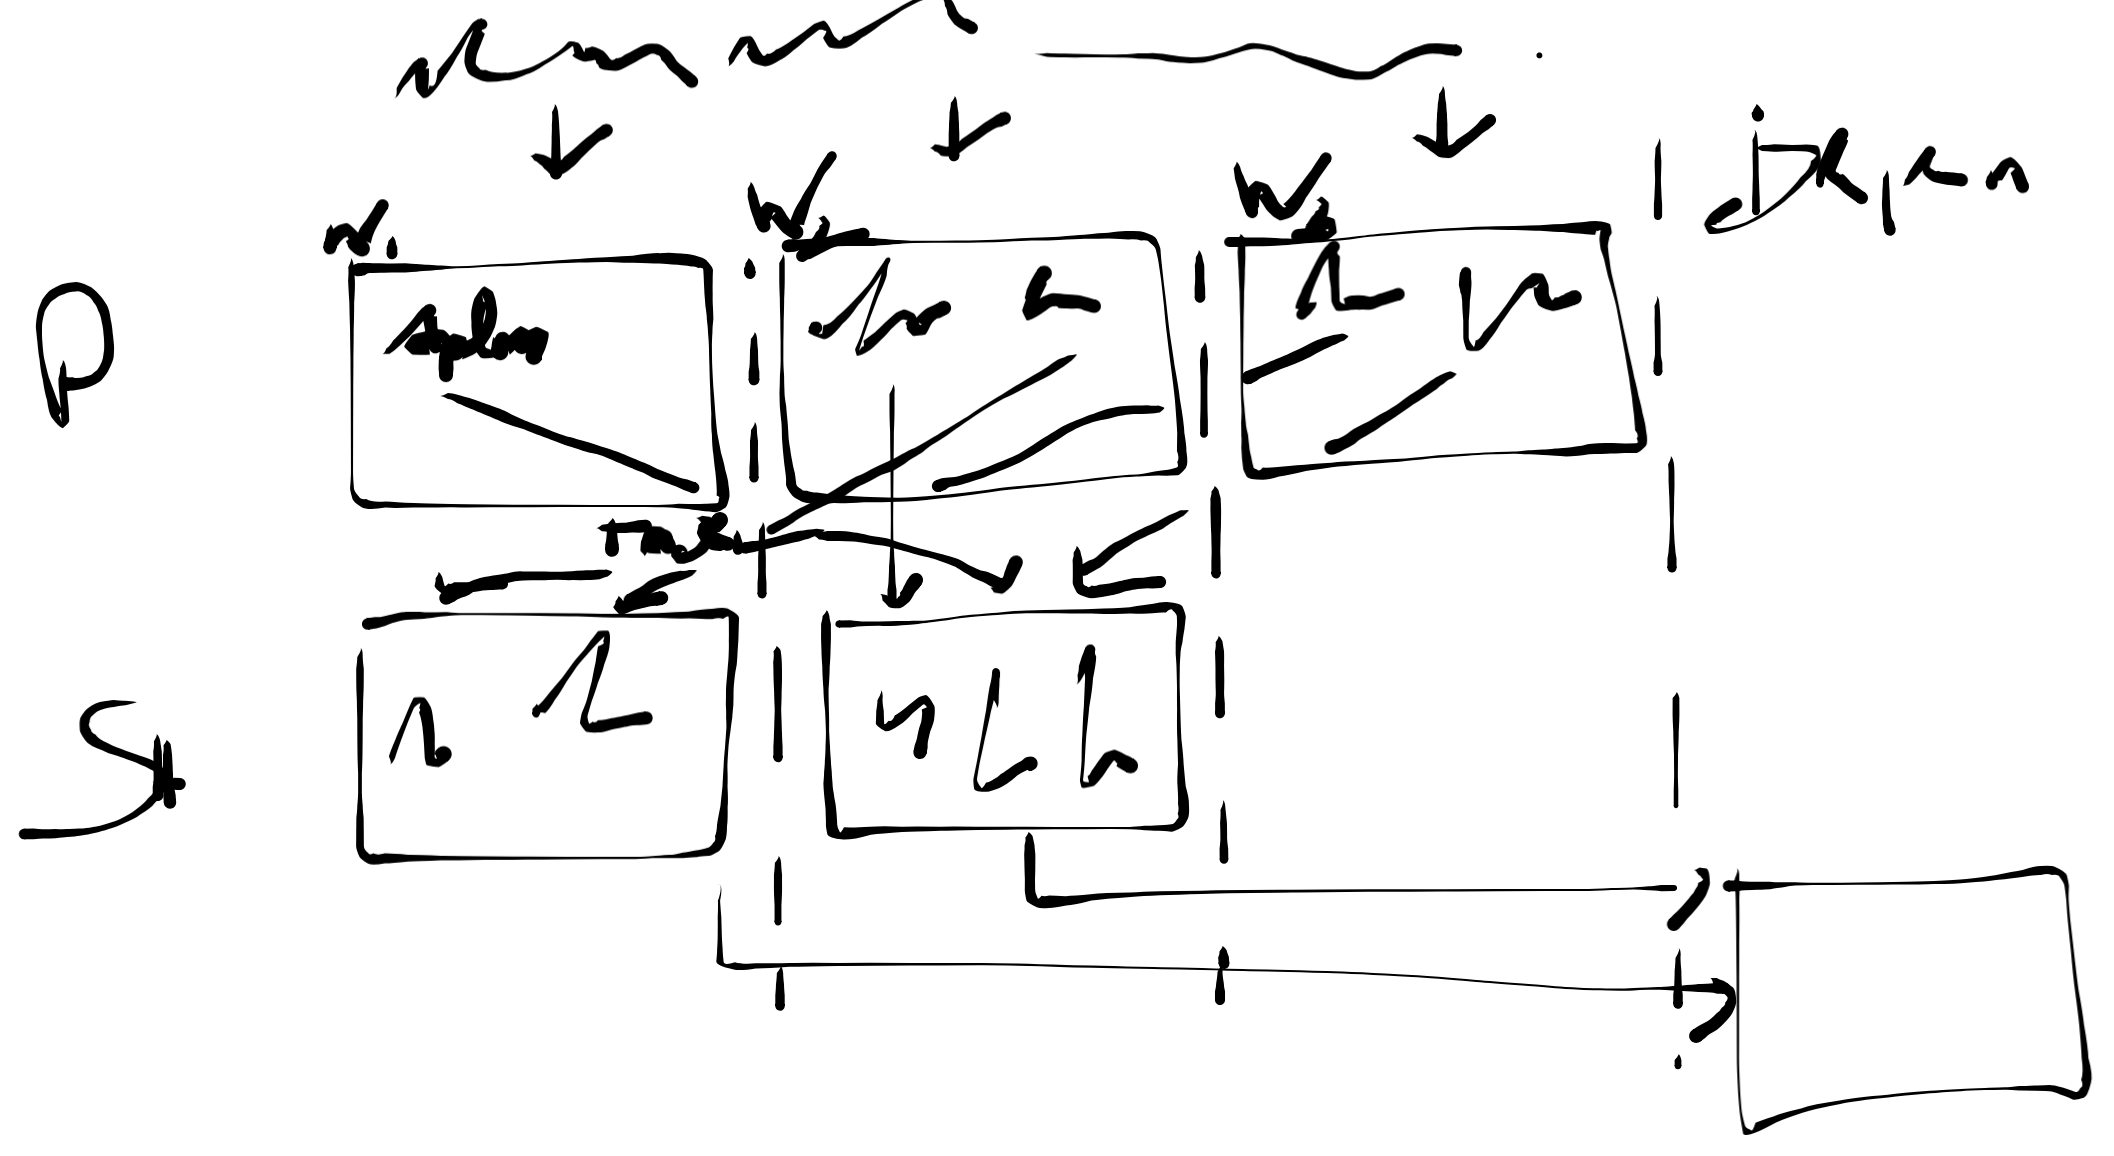
\includegraphics[width=29.36in]{images/07-tuning-spark-rdds} 

}

\caption{Spark RDDs}\label{fig:unnamed-chunk-60}
\end{figure}

\begin{Shaded}
\begin{Highlighting}[]
\NormalTok{sc <-}\StringTok{ }\KeywordTok{spark_connect}\NormalTok{(}\DataTypeTok{master =} \StringTok{"local"}\NormalTok{, }\DataTypeTok{memory =} \StringTok{"4g"}\NormalTok{, }\DataTypeTok{cores =} \DecValTok{8}\NormalTok{)}

\NormalTok{entries <-}\StringTok{ }\DecValTok{100000000}
\NormalTok{sort_r <-}\StringTok{ }\KeywordTok{system.time}\NormalTok{(}\KeywordTok{runif}\NormalTok{(entries, }\DecValTok{0}\NormalTok{, }\DecValTok{100}\NormalTok{) }\OperatorTok\StringTok{ }\KeywordTok{sort}\NormalTok{())[}\StringTok{"elapsed"}\NormalTok{]}
\NormalTok{sort_spark <-}\StringTok{ }\KeywordTok{system.time}\NormalTok{(}\KeywordTok{sdf_len}\NormalTok{(sc, entries) }\OperatorTok\StringTok{ }\NormalTok{dplyr}\OperatorTok{::}\KeywordTok{mutate}\NormalTok{(}\DataTypeTok{x =} \KeywordTok{rand}\NormalTok{()) }\OperatorTok\StringTok{ }\NormalTok{dplyr}\OperatorTok{::}\KeywordTok{arrange}\NormalTok{() }\OperatorTok\StringTok{ }\NormalTok{dplyr}\OperatorTok{::}\KeywordTok{compute}\NormalTok{())[}\StringTok{"elapsed"}\NormalTok{]}

\KeywordTok{lapply}\NormalTok{(}\KeywordTok{expt}\NormalTok{(}\DecValTok{1}\OperatorTok{:}\DecValTok{10}\NormalTok{))}
\end{Highlighting}
\end{Shaded}

\hypertarget{configuration}{%
\section{Configuration}\label{configuration}}

\begin{Shaded}
\begin{Highlighting}[]
\NormalTok{config <-}\StringTok{ }\KeywordTok{spark_config}\NormalTok{()}
\NormalTok{sc <-}\StringTok{ }\KeywordTok{spark_connect}\NormalTok{(}\DataTypeTok{master =} \StringTok{"local"}\NormalTok{)}

\KeywordTok{spark_context_config}\NormalTok{(sc)}

\KeywordTok{spark_session_config}\NormalTok{(sc)}

\CommentTok{# Previous versions}
\KeywordTok{spark_hive_config}\NormalTok{(sc)}
\end{Highlighting}
\end{Shaded}

\url{https://spark.apache.org/docs/latest/configuration.html}

\hypertarget{caching}{%
\section{Caching}\label{caching}}

Most sparklyr operations that retrieve a Spark data frame, cache the
results in-memory, for instance, running \texttt{spark\_read\_parquet()}
or \texttt{sdf\_copy\_to()} will provide a Spark dataframe that is
already cached in-memory. As a Spark data frame, this object can be used
in most sparklyr functions, including data analysis with dplyr or
machine learning.

\begin{Shaded}
\begin{Highlighting}[]
\KeywordTok{library}\NormalTok{(sparklyr)}
\NormalTok{sc <-}\StringTok{ }\KeywordTok{spark_connect}\NormalTok{(}\DataTypeTok{master =} \StringTok{"local"}\NormalTok{)}
\end{Highlighting}
\end{Shaded}

\begin{Shaded}
\begin{Highlighting}[]
\NormalTok{iris_tbl <-}\StringTok{ }\KeywordTok{sdf_copy_to}\NormalTok{(sc, iris, }\DataTypeTok{overwrite =} \OtherTok{TRUE}\NormalTok{)}
\end{Highlighting}
\end{Shaded}

You can inspect which tables are cached by navigating to the Spark UI
using \texttt{spark\_web(sc)}, opening the storage tab, and clicking on
a given RDD:

\begin{figure}

{\centering 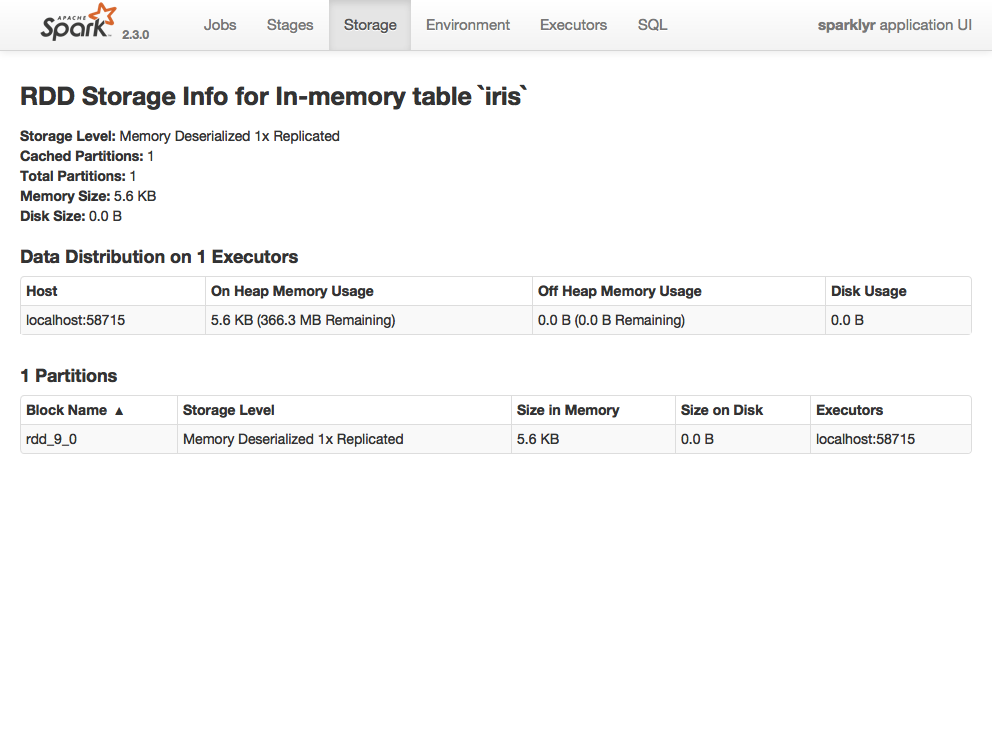
\includegraphics[width=13.78in]{images/07-tuning-cache-rdd-web} 

}

\caption{Cached RDD in Spark Web Interface.}\label{fig:spark-standalone-rdd-web}
\end{figure}

Data loaded in memory will be released when the R session terminates
either explicitly or implicitly with a restart or disconnection;
however, to free up resources, you can use \texttt{tbl\_uncache()}:

\begin{Shaded}
\begin{Highlighting}[]
\KeywordTok{tbl_uncache}\NormalTok{(sc, }\StringTok{"iris"}\NormalTok{)}
\end{Highlighting}
\end{Shaded}

\hypertarget{partitions}{%
\section{Partitions}\label{partitions}}

\hypertarget{shuffling}{%
\section{Shuffling}\label{shuffling}}

\hypertarget{checkpointing}{%
\section{Checkpointing}\label{checkpointing}}

\hypertarget{troubleshooting-1}{%
\section{Troubleshooting}\label{troubleshooting-1}}

\hypertarget{graph-visualization}{%
\subsection{Graph Visualization}\label{graph-visualization}}

\begin{figure}

{\centering 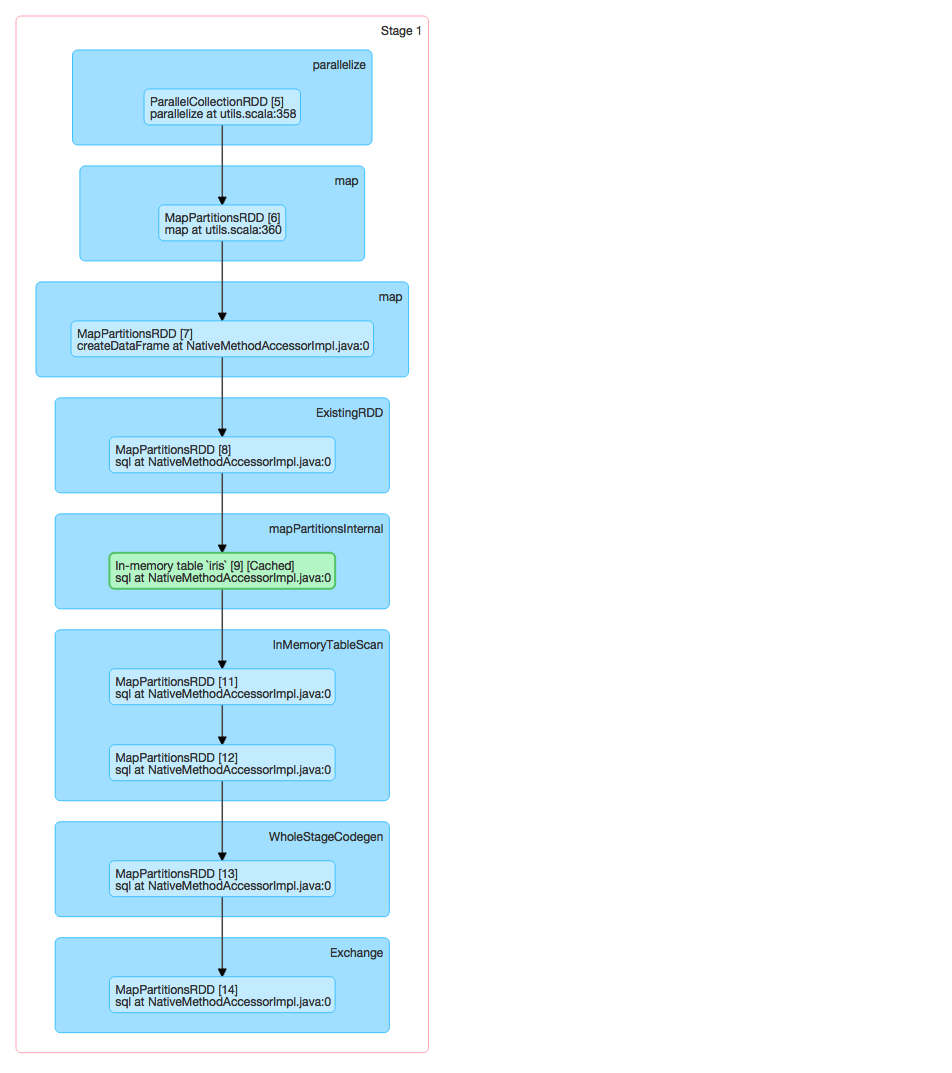
\includegraphics[width=13.22in]{images/07-tuning-spark-graph-visualization} 

}

\caption{Spark Graph Visualization}\label{fig:unnamed-chunk-69}
\end{figure}

\hypertarget{event-timeline}{%
\subsection{Event Timeline}\label{event-timeline}}

One of the best ways to tune your Spark jobs is to use the Spark's
\href{spark-web-interface}{web interface}, click on the job being
diagnosed, then the stage and then expand the \textbf{event timeline}.

Lets the take a look at the event timeline for the ordering a data frame
by a given column using three partitions:

\begin{Shaded}
\begin{Highlighting}[]
\KeywordTok{spark_connect}\NormalTok{(}\DataTypeTok{master =} \StringTok{"local"}\NormalTok{) }\OperatorTok
\StringTok{  }\KeywordTok{copy_to}\NormalTok{(iris, }\DataTypeTok{repartition =} \DecValTok{3}\NormalTok{) }\OperatorTok
\StringTok{  }\KeywordTok{arrange}\NormalTok{(Sepal_Width)}
\end{Highlighting}
\end{Shaded}

\begin{figure}

{\centering 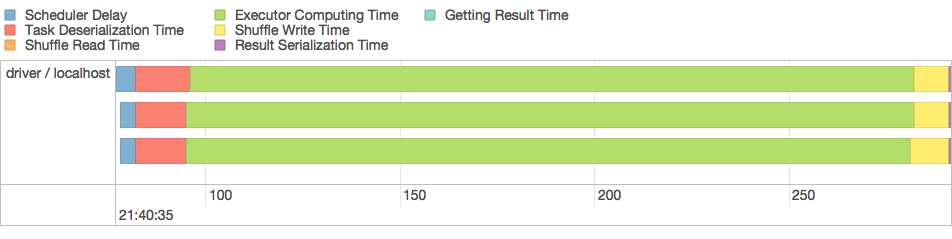
\includegraphics[width=0.9\linewidth]{images/07-tuning-spark-event-timeline} 

}

\caption{Spark Event Timeline}\label{fig:unnamed-chunk-73}
\end{figure}

\hypertarget{recap-3}{%
\section{Recap}\label{recap-3}}

\hypertarget{extensions}{%
\chapter{Extensions}\label{extensions}}

While \textbf{this chatper has not been written.}, a few resources are
available to help explore these topics until this chapter gets written.

\hypertarget{using-extensions}{%
\section{Using Extensions}\label{using-extensions}}

\hypertarget{graphframes}{%
\subsection{GraphFrames}\label{graphframes}}

See
\href{http://spark.rstudio.com/graphframes/}{spark.rstudio.com/graphframes}.

\hypertarget{mleap}{%
\subsection{Mleap}\label{mleap}}

See
\href{http://spark.rstudio.com/guides/mleap/}{spark.rstudio.com/guides/mleap}.

\hypertarget{h2o}{%
\subsection{H2O}\label{h2o}}

See
\href{http://spark.rstudio.com/guides/h2o/}{spark.rstudio.com/guides/h2o}.

\hypertarget{writting-extensions}{%
\section{Writting Extensions}\label{writting-extensions}}

See
\href{http://spark.rstudio.com/extensions/}{spark.rstudio.com/extensions}.

\hypertarget{rstudio-projects}{%
\subsection{RStudio Projects}\label{rstudio-projects}}

\hypertarget{distributed}{%
\chapter{Distributed R}\label{distributed}}

While \textbf{this chatper has not been written.}, use
\href{http://spark.rstudio.com/guides/distributed-r/}{spark.rstudio.com/guides/distributed-r}
to learn how to use R directly over each worker node.

\hypertarget{use-cases}{%
\section{Use Cases}\label{use-cases}}

\hypertarget{grouping}{%
\section{Grouping}\label{grouping}}

\hypertarget{packages}{%
\section{Packages}\label{packages}}

\hypertarget{restrictions}{%
\section{Restrictions}\label{restrictions}}

\hypertarget{troubleshooting-2}{%
\section{Troubleshooting}\label{troubleshooting-2}}

\hypertarget{streaming}{%
\chapter{Streaming}\label{streaming}}

\hypertarget{overview-4}{%
\section{Overview}\label{overview-4}}

One can understand a stream as an unbounded data frame, meaning, a data
frame with finite columns but infinite rows. Streams are most relevant
when processing real time data; for example, when analyzing a Twitter
feed or stock prices. Both examples have well defined columns, like
`tweet' or `price', but there are always new rows of data to be
analyzed.

Spark provided initial support for streams with Spark's DStreams;
however, a more versatile and efficient replacement is available through
\href{https://spark.apache.org/docs/latest/structured-streaming-programming-guide.html}{Spark
structured streams}. Structured streams provide scalable and
fault-torerant data processing over streams of data. That means, one can
use many machines to process multiple streaming sources, perform joins
with other streams or static sources, and recover from failures with
at-least-once guarantees (where each message is certain to be delivered,
but may do so multiple times).

In order to use structured streams in \texttt{sparklyr}, one needs to
define the \textbf{sources}, \textbf{transformations} and a
\textbf{destination}:

\begin{itemize}
\tightlist
\item
  The \textbf{sources} are defined using any of the
  \texttt{stream\_read\_*()} functions to read streams of data from
  various data sources.
\item
  The \textbf{transformations} can be specified using \texttt{dplyr},
  \texttt{SQL}, scoring pipelines or R code through
  \texttt{spark\_apply()}.
\item
  The \textbf{destination} is defined with the
  \texttt{stream\_write\_*()} functions, it often also referenced as a
  sink.
\end{itemize}

Since the transformation step is optional, the simplest stream we can
define is to continuously process files, which would effectively copy
text files between source and destination. We can define this
copy-stream in \texttt{sparklyr} as follows:

\begin{Shaded}
\begin{Highlighting}[]
\KeywordTok{library}\NormalTok{(sparklyr)}
\NormalTok{sc <-}\StringTok{ }\KeywordTok{spark_connect}\NormalTok{(}\DataTypeTok{master =} \StringTok{"local"}\NormalTok{)}
\NormalTok{stream <-}\StringTok{ }\KeywordTok{stream_read_text}\NormalTok{(sc, }\StringTok{"source/"}\NormalTok{) }\OperatorTok\StringTok{ }\KeywordTok{stream_write_text}\NormalTok{(}\StringTok{"destination/"}\NormalTok{)}
\end{Highlighting}
\end{Shaded}

The streams starts running with \texttt{stream\_write\_*()}; once
executed, the stream will monitor the \texttt{source} path and process
data into the \texttt{destination/} path as it arrives. We can use
\texttt{view\_stream()} to track the \textbf{rows per second (rps)}
being processed in the source, destination and their latest values over
time:

\begin{Shaded}
\begin{Highlighting}[]
\KeywordTok{stream_view}\NormalTok{(stream)}
\end{Highlighting}
\end{Shaded}

\begin{figure}

{\centering \includegraphics[width=1\linewidth,height=280pt]{the-r-in-spark_files/figure-latex/unnamed-chunk-78-1} 

}

\caption{Viewing a Spark Stream with sparklyr}\label{fig:unnamed-chunk-78}
\end{figure}

Notice that the rows-per-second in the destination stream are higher
than the rows-per-second in the source stream; this is expected and
desireable since Spark measures incoming rates from the source, but
actual row processing times in the destination stream.

Use \texttt{stream\_stop()} to properly stop processing data from this
stream:

\begin{Shaded}
\begin{Highlighting}[]
\KeywordTok{stream_stop}\NormalTok{(stream)}
\end{Highlighting}
\end{Shaded}

In order to reproduce the above example, one needs to feed streaming
data into the \texttt{source/} path. This was accomplished by running,
before \texttt{stream\_view(stream)}, the following script to produce a
file every second containing lines of text that follow two overlapping
binomial distributions. In practice, you would connect to existing
sources without having to generate data artificially.

\begin{Shaded}
\begin{Highlighting}[]
\KeywordTok{unlink}\NormalTok{(}\KeywordTok{c}\NormalTok{(}\StringTok{"source/"}\NormalTok{, }\StringTok{"destination/"}\NormalTok{), }\DataTypeTok{recursive =} \OtherTok{TRUE}\NormalTok{)}
\KeywordTok{dir.create}\NormalTok{(}\StringTok{"source"}\NormalTok{)}
\NormalTok{callr}\OperatorTok{::}\KeywordTok{r_bg}\NormalTok{(}\ControlFlowTok{function}\NormalTok{() \{}
\NormalTok{  dist <-}\StringTok{ }\KeywordTok{floor}\NormalTok{(}\DecValTok{10} \OperatorTok{+}\StringTok{ }\FloatTok{1e5} \OperatorTok{*}\StringTok{ }\NormalTok{(}\KeywordTok{dbinom}\NormalTok{(}\DecValTok{1}\OperatorTok{:}\DecValTok{50}\NormalTok{, }\DecValTok{50}\NormalTok{, }\FloatTok{0.7}\NormalTok{) }\OperatorTok{+}\StringTok{ }\KeywordTok{dbinom}\NormalTok{(}\DecValTok{1}\OperatorTok{:}\DecValTok{50}\NormalTok{, }\DecValTok{50}\NormalTok{, }\FloatTok{0.3}\NormalTok{)))}
  \ControlFlowTok{for}\NormalTok{ (i }\ControlFlowTok{in} \KeywordTok{seq_len}\NormalTok{(}\DecValTok{10}\NormalTok{)) \{}
    \KeywordTok{writeLines}\NormalTok{(}\KeywordTok{paste}\NormalTok{(}\StringTok{"Row"}\NormalTok{, }\DecValTok{1}\OperatorTok{:}\NormalTok{dist[i]), }\KeywordTok{paste0}\NormalTok{(}\StringTok{"source/hello_"}\NormalTok{, i, }\StringTok{".txt"}\NormalTok{))}
    \KeywordTok{Sys.sleep}\NormalTok{(}\DecValTok{1}\NormalTok{)}
\NormalTok{  \}}
\NormalTok{\})}
\end{Highlighting}
\end{Shaded}

For the subsequent examples, a stream with one hundred rows of text will
be used:

\begin{Shaded}
\begin{Highlighting}[]
\KeywordTok{writeLines}\NormalTok{(}\KeywordTok{paste}\NormalTok{(}\StringTok{"Row"}\NormalTok{, }\DecValTok{1}\OperatorTok{:}\DecValTok{100}\NormalTok{), }\StringTok{"source/rows.txt"}\NormalTok{)}
\end{Highlighting}
\end{Shaded}

\hypertarget{transformations}{%
\section{Transformations}\label{transformations}}

Streams can be transformed using \texttt{dplyr}, SQL, pipelines or R
code. We can use as many transformations as needed in the same way that
Spark data frames can be transformed with \texttt{sparklyr}. The
transformation source can be streams or data frames but the output is
always a stream. If needed, one can always take a snapshot from the
destination stream and save the output as a data frame, which is what
\texttt{sparklyr} will do for you if a destination stream is not
specified. Conceptually, this looks as follows:

\begin{figure}

{\centering \includegraphics[width=1\linewidth,height=280pt]{the-r-in-spark_files/figure-latex/unnamed-chunk-82-1} 

}

\caption{Streams Transformation Diagram}\label{fig:unnamed-chunk-82}
\end{figure}

\hypertarget{streams-dplyr}{%
\subsection{dplyr}\label{streams-dplyr}}

Using \texttt{dplyr}, we can process each row of the stream; for
example, we can filter the stream to only the rows containing a number
one:

\begin{Shaded}
\begin{Highlighting}[]
\KeywordTok{library}\NormalTok{(dplyr, }\DataTypeTok{warn.conflicts =} \OtherTok{FALSE}\NormalTok{)}

\KeywordTok{stream_read_text}\NormalTok{(sc, }\StringTok{"source/"}\NormalTok{) }\OperatorTok
\StringTok{  }\KeywordTok{filter}\NormalTok{(text }\OperatorTok\StringTok{ "%1%"}\NormalTok{)}
\end{Highlighting}
\end{Shaded}

\begin{verbatim}
## # Source:   lazy query [?? x 1]
## # Database: spark_connection
##    text  
##    <chr> 
##  1 Row 1 
##  2 Row 10
##  3 Row 11
##  4 Row 12
##  5 Row 13
##  6 Row 14
##  7 Row 15
##  8 Row 16
##  9 Row 17
## 10 Row 18
## # ... with more rows
\end{verbatim}

Since the destination was not specified, \texttt{sparklyr} creates a
temporary memory stream and previews the contents of a stream by
capturing a few seconds of streaming data.

We can also aggregate data with \texttt{dplyr},

\begin{Shaded}
\begin{Highlighting}[]
\KeywordTok{stream_read_text}\NormalTok{(sc, }\StringTok{"source/"}\NormalTok{) }\OperatorTok
\StringTok{  }\KeywordTok{summarise}\NormalTok{(}\DataTypeTok{n =} \KeywordTok{n}\NormalTok{())}
\end{Highlighting}
\end{Shaded}

\begin{verbatim}
## # Source:   lazy query [?? x 1]
## # Database: spark_connection
##       n
##   <dbl>
## 1   100
\end{verbatim}

and even join across many concurrent streams:

\begin{Shaded}
\begin{Highlighting}[]
\KeywordTok{left_join}\NormalTok{(}
  \KeywordTok{stream_read_text}\NormalTok{(sc, }\StringTok{"source/"}\NormalTok{) }\OperatorTok\StringTok{ }\KeywordTok{stream_watermark}\NormalTok{(),}
  \KeywordTok{stream_read_text}\NormalTok{(sc, }\StringTok{"source/"}\NormalTok{) }\OperatorTok\StringTok{ }\KeywordTok{stream_watermark}\NormalTok{() }\OperatorTok\StringTok{ }\KeywordTok{mutate}\NormalTok{(}\DataTypeTok{random =} \KeywordTok{rand}\NormalTok{()),}
\NormalTok{)}
\end{Highlighting}
\end{Shaded}

\begin{verbatim}
## Joining, by = c("text", "timestamp")
\end{verbatim}

\begin{verbatim}
## # Source:   lazy query [?? x 3]
## # Database: spark_connection
##    text   timestamp           random
##    <chr>  <dttm>               <dbl>
##  1 Row 8  2018-07-16 17:23:05  0.108
##  2 Row 15 2018-07-16 17:23:05  0.965
##  3 Row 16 2018-07-16 17:23:05  0.171
##  4 Row 20 2018-07-16 17:23:05  0.282
##  5 Row 22 2018-07-16 17:23:05  0.868
##  6 Row 27 2018-07-16 17:23:05  0.660
##  7 Row 35 2018-07-16 17:23:05  0.492
##  8 Row 38 2018-07-16 17:23:05  0.609
##  9 Row 39 2018-07-16 17:23:05  0.461
## 10 Row 48 2018-07-16 17:23:05  0.342
## # ... with more rows
\end{verbatim}

However, some operations, require watermarks to define when to stop
waiting for late data. You can specify watermarks in \texttt{sparklyr}
using \texttt{stream\_watermak()}, see also
\href{https://spark.apache.org/docs/latest/structured-streaming-programming-guide.html\#handling-late-data-and-watermarking}{handling
late data} in Spark's documentation.

\hypertarget{streams-pipelines}{%
\subsection{Pipelines}\label{streams-pipelines}}

Spark pipelines can be used for scoring streams, but not to train over
streaming data. The former is fully supported while the latter is a
feature under active development by the Spark community.

To use a pipeline for scoring a stream, first train a Spark pipeline
over a static dataset. Once trained, save the pipeline, then reload and
score over a stream as follows:

\begin{Shaded}
\begin{Highlighting}[]
\NormalTok{fitted_pipeline <-}\StringTok{ }\KeywordTok{ml_load}\NormalTok{(sc, }\StringTok{"iris-fitted/"}\NormalTok{)}

\KeywordTok{stream_read_csv}\NormalTok{(sc, }\StringTok{"iris-in"}\NormalTok{) }\OperatorTok
\StringTok{  }\KeywordTok{sdf_transform}\NormalTok{(fitted_pipeline) }\OperatorTok
\StringTok{  }\KeywordTok{stream_write_csv}\NormalTok{(}\StringTok{"iris-out"}\NormalTok{)}
\end{Highlighting}
\end{Shaded}

\hypertarget{streams-r}{%
\subsection{R Code}\label{streams-r}}

Arbitrary R code can also be used to transform a stream with the use of
\texttt{spark\_apply()}. Following the same principles from executing R
code over Spark data frames, for structured streams,
\texttt{spark\_apply()} runs R code over each executor in the cluster
where data is available, this enables processing high-throughput streams
and fullfill low-latency requirements.

The following example splits a stream of \texttt{Row\ \#} line entries
and adds jitter using R code:

\begin{Shaded}
\begin{Highlighting}[]
\KeywordTok{stream_read_text}\NormalTok{(sc, }\StringTok{"source/"}\NormalTok{) }\OperatorTok
\StringTok{  }\KeywordTok{spark_apply}\NormalTok{(}\ControlFlowTok{function}\NormalTok{(df) \{}
    \KeywordTok{data.frame}\NormalTok{(}
      \DataTypeTok{data =} \KeywordTok{jitter}\NormalTok{(}\KeywordTok{as.numeric}\NormalTok{(}\KeywordTok{gsub}\NormalTok{(}\StringTok{"Row "}\NormalTok{, }\StringTok{""}\NormalTok{, df}\OperatorTok{$}\NormalTok{text)))}
\NormalTok{    )}
\NormalTok{  \})}
\end{Highlighting}
\end{Shaded}

\begin{verbatim}
## # Source:   table<sparklyr_tmp_781e6cb21c24> [?? x 1]
## # Database: spark_connection
##      data
##     <dbl>
##  1  0.866
##  2  1.95 
##  3  2.92 
##  4  3.92 
##  5  5.09 
##  6  6.16 
##  7  6.94 
##  8  8.15 
##  9  8.81 
## 10 10.1  
## # ... with more rows
\end{verbatim}

\hypertarget{shiny}{%
\section{Shiny}\label{shiny}}

Streams can be used with Shiny by making use of the
\texttt{reactiveSpark()} to retrieve the stream as a reactive data
source. Internally, \texttt{reactiveSpark()} makes use of
\href{https://shiny.rstudio.com/reference/shiny/latest/reactivePoll.html}{reactivePoll()}
to check the stream's timestamp and collect the stream contents when
needed.

The following Shiny application makes use of \texttt{reactiveSpark()} to
view a Spark stream summarized with \texttt{dplyr}:

\begin{Shaded}
\begin{Highlighting}[]
\KeywordTok{library}\NormalTok{(shiny)}
\KeywordTok{library}\NormalTok{(sparklyr)}
\KeywordTok{library}\NormalTok{(dplyr)}

\NormalTok{sc <-}\StringTok{ }\KeywordTok{spark_connect}\NormalTok{(}\DataTypeTok{master =} \StringTok{"local"}\NormalTok{)}

\NormalTok{ui <-}\StringTok{ }\KeywordTok{fluidPage}\NormalTok{(}
  \KeywordTok{sidebarLayout}\NormalTok{(}
    \KeywordTok{mainPanel}\NormalTok{(}
      \KeywordTok{tableOutput}\NormalTok{(}\StringTok{"table"}\NormalTok{)}
\NormalTok{    )}
\NormalTok{  )}
\NormalTok{)}

\NormalTok{server <-}\StringTok{ }\ControlFlowTok{function}\NormalTok{(input, output, session) \{}
\NormalTok{  pollData <-}\StringTok{ }\KeywordTok{stream_read_text}\NormalTok{(sc, }\StringTok{"source/"}\NormalTok{) }\OperatorTok
\StringTok{    }\KeywordTok{summarise}\NormalTok{(}\DataTypeTok{n =} \KeywordTok{n}\NormalTok{()) }\OperatorTok
\StringTok{    }\KeywordTok{reactiveSpark}\NormalTok{(}\DataTypeTok{session =}\NormalTok{ session)}

\NormalTok{  output}\OperatorTok{$}\NormalTok{table <-}\StringTok{ }\KeywordTok{renderTable}\NormalTok{(\{}
    \KeywordTok{pollData}\NormalTok{()}
\NormalTok{  \})}
\NormalTok{\}}

\KeywordTok{shinyApp}\NormalTok{(}\DataTypeTok{ui =}\NormalTok{ ui, }\DataTypeTok{server =}\NormalTok{ server)}
\end{Highlighting}
\end{Shaded}

\hypertarget{formats}{%
\section{Formats}\label{formats}}

The following formats are available to read and write streaming data:

\begin{longtable}[]{@{}lll@{}}
\toprule
Format & Read & Write\tabularnewline
\midrule
\endhead
CSV & stream\_read\_csv & stream\_write\_csv\tabularnewline
JDBC & stream\_read\_jdbc & stream\_write\_jdbc\tabularnewline
JSON & stream\_read\_json & stream\_write\_json\tabularnewline
Kafka & stream\_read\_kafka & stream\_write\_kafka\tabularnewline
ORC & stream\_read\_orc & stream\_write\_orc\tabularnewline
Parquet & stream\_read\_parquet & stream\_write\_parquet\tabularnewline
Text & stream\_read\_text & stream\_write\_text\tabularnewline
Memory & & stream\_write\_memory\tabularnewline
\bottomrule
\end{longtable}

\hypertarget{contributing}{%
\chapter{Contributing}\label{contributing}}

\textbf{This chatper has not been written.}

While there are many ways to contribute to \texttt{sparklyr} from
helping community members to opening github issues, this chapter focuses
on those readers interested in contributing fixes and features to
\texttt{sparklyr} but will also help those who want to understand how
\texttt{sparklyr} works internally.

\hypertarget{overview-5}{%
\section{Overview}\label{overview-5}}

(architecture overview)

\hypertarget{serialization}{%
\section{Serialization}\label{serialization}}

\hypertarget{invocations}{%
\section{Invocations}\label{invocations}}

\hypertarget{r-packages}{%
\section{R Packages}\label{r-packages}}

(dbi, dplyr, broom, etc)

\hypertarget{connections-1}{%
\section{Connections}\label{connections-1}}

\hypertarget{distributed-r}{%
\section{Distributed R}\label{distributed-r}}

\hypertarget{appendix}{%
\chapter*{Appendix}\label{appendix}}
\addcontentsline{toc}{chapter}{Appendix}

\hypertarget{storage-capacity}{%
\section{Worlds Store Capacity}\label{storage-capacity}}

\begin{Shaded}
\begin{Highlighting}[]
\KeywordTok{library}\NormalTok{(tidyverse)}
\KeywordTok{read_csv}\NormalTok{(}\StringTok{"data/01-worlds-capacity-to-store-information.csv"}\NormalTok{, }\DataTypeTok{skip =} \DecValTok{8}\NormalTok{) }\OperatorTok
\StringTok{  }\KeywordTok{gather}\NormalTok{(}\DataTypeTok{key =}\NormalTok{ storage, }\DataTypeTok{value =}\NormalTok{ capacity, analog, digital) }\OperatorTok
\StringTok{  }\KeywordTok{mutate}\NormalTok{(}\DataTypeTok{year =}\NormalTok{ X1, }\DataTypeTok{terabytes =}\NormalTok{ capacity }\OperatorTok{/}\StringTok{ }\FloatTok{1e+12}\NormalTok{) }\OperatorTok
\StringTok{  }\KeywordTok{ggplot}\NormalTok{(}\KeywordTok{aes}\NormalTok{(}\DataTypeTok{x =}\NormalTok{ year, }\DataTypeTok{y =}\NormalTok{ terabytes, }\DataTypeTok{group =}\NormalTok{ storage)) }\OperatorTok{+}
\StringTok{    }\KeywordTok{geom_line}\NormalTok{(}\KeywordTok{aes}\NormalTok{(}\DataTypeTok{linetype =}\NormalTok{ storage)) }\OperatorTok{+}
\StringTok{    }\KeywordTok{geom_point}\NormalTok{(}\KeywordTok{aes}\NormalTok{(}\DataTypeTok{shape =}\NormalTok{ storage)) }\OperatorTok{+}
\StringTok{    }\KeywordTok{scale_y_log10}\NormalTok{(}
      \DataTypeTok{breaks =}\NormalTok{ scales}\OperatorTok{::}\KeywordTok{trans_breaks}\NormalTok{(}\StringTok{"log10"}\NormalTok{, }\ControlFlowTok{function}\NormalTok{(x) }\DecValTok{10}\OperatorTok{^}\NormalTok{x),}
      \DataTypeTok{labels =}\NormalTok{ scales}\OperatorTok{::}\KeywordTok{trans_format}\NormalTok{(}\StringTok{"log10"}\NormalTok{, scales}\OperatorTok{::}\KeywordTok{math_format}\NormalTok{(}\DecValTok{10}\OperatorTok{^}\NormalTok{x))}
\NormalTok{    ) }\OperatorTok{+}
\StringTok{    }\KeywordTok{theme_light}\NormalTok{() }\OperatorTok{+}
\StringTok{    }\KeywordTok{theme}\NormalTok{(}\DataTypeTok{legend.position =} \StringTok{"bottom"}\NormalTok{)}
\end{Highlighting}
\end{Shaded}

\hypertarget{cran-downloads}{%
\section{Daily downloads of CRAN packages}\label{cran-downloads}}

\begin{Shaded}
\begin{Highlighting}[]
\NormalTok{downloads_csv <-}\StringTok{ "data/01-intro-r-cran-downloads.csv"}
\ControlFlowTok{if}\NormalTok{ (}\OperatorTok{!}\KeywordTok{file.exists}\NormalTok{(downloads_csv)) \{}
\NormalTok{  downloads <-}\StringTok{ }\NormalTok{cranlogs}\OperatorTok{::}\KeywordTok{cran_downloads}\NormalTok{(}\DataTypeTok{from =} \StringTok{"2014-01-01"}\NormalTok{, }\DataTypeTok{to =} \StringTok{"2018-01-01"}\NormalTok{)}
\NormalTok{  readr}\OperatorTok{::}\KeywordTok{write_csv}\NormalTok{(downloads, downloads_csv)}
\NormalTok{\}}

\NormalTok{cran_downloads <-}\StringTok{ }\NormalTok{readr}\OperatorTok{::}\KeywordTok{read_csv}\NormalTok{(downloads_csv)}

\KeywordTok{ggplot}\NormalTok{(cran_downloads, }\KeywordTok{aes}\NormalTok{(date, count)) }\OperatorTok{+}\StringTok{ }
\StringTok{  }\KeywordTok{geom_point}\NormalTok{(}\DataTypeTok{colour=}\StringTok{"black"}\NormalTok{, }\DataTypeTok{pch =} \DecValTok{21}\NormalTok{, }\DataTypeTok{size =} \DecValTok{1}\NormalTok{) }\OperatorTok{+}
\StringTok{  }\KeywordTok{scale_x_date}\NormalTok{() }\OperatorTok{+}
\StringTok{  }\KeywordTok{xlab}\NormalTok{(}\StringTok{""}\NormalTok{) }\OperatorTok{+}
\StringTok{  }\KeywordTok{ylab}\NormalTok{(}\StringTok{""}\NormalTok{) }\OperatorTok{+}
\StringTok{  }\KeywordTok{theme_light}\NormalTok{()}
\end{Highlighting}
\end{Shaded}

\hypertarget{cluster-trends}{%
\section{Google trends for mainframes, cloud computing and
kubernetes}\label{cluster-trends}}

\begin{Shaded}
\begin{Highlighting}[]
\KeywordTok{library}\NormalTok{(r2d3)}

\KeywordTok{read.csv}\NormalTok{(}\StringTok{"data/05-cluster-trends.csv"}\NormalTok{) }\OperatorTok
\StringTok{  }\KeywordTok{mutate}\NormalTok{(}\DataTypeTok{month =} \KeywordTok{as.Date}\NormalTok{(}\KeywordTok{paste}\NormalTok{(month, }\StringTok{"-01"}\NormalTok{, }\DataTypeTok{sep =} \StringTok{""}\NormalTok{))) }\OperatorTok
\StringTok{  }\KeywordTok{r2d3}\NormalTok{(}\DataTypeTok{script=}\StringTok{"images/05-clusters-trends.js"}\NormalTok{)}
\end{Highlighting}
\end{Shaded}

\bibliography{book.bib,packages.bib}


\end{document}
